\chapter{Security Analysis}
\label{sec:security_analyse}

% Ist das zentrale Kapitel der Arbeit. Hier werden das Ziel sowie die
% eigenen Ideen, Wertungen, Entwurfsentscheidungen vorgebracht. Es kann
% sich lohnen, verschiedene Möglichkeiten durchzuspielen und dann
% explizit zu begründen, warum man sich für eine bestimmte entschieden
% hat. Dieses Kapitel sollte - zumindest in Stichworten - schon bei den
% ersten Festlegungen eines Entwurfs skizziert werden.
% Es wird sich aber in einer normal verlaufenden
% Arbeit dauernd etwas daran ändern. Das Kapitel darf nicht zu
% detailliert werden, sonst langweilt sich der Leser. Es ist sehr
% wichtig, das richtige Abstraktionsniveau zu finden. Beim Verfassen
% sollte man auf die Wiederverwendbarkeit des Textes achten.

% Plant man eine Veröffentlichung aus der Arbeit zu machen, können von
% diesem Kapitel Teile genommen werden. Das Kapitel wird in der Regel
% wohl mindestens 8 Seiten haben, mehr als 20 können ein Hinweis darauf
% sein, daß das Abstraktionsniveau verfehlt wurde.

%\ldots design \ldots

%\todo{write design}
This chapter aims to analyze the potential vulnerabilities in the OCI runtime interface~\cite*{oci-runtime-spec} through which an adversary can obtain sensitive data of an application. The first section defines the threat model (Section~\ref{sec:Threat_model}). Subsequently, Section~\ref{sec:security_analyse_oci_analysis} explores the problems in the OCI runtime interface~\cite*{oci-runtime-spec} in the 
context of confidential computing. Section~\ref{sec:security_analyse_quark_analysis} then uses the vulnerabilities found in the OCI runtime interface to conduct a security analysis of Quark~\cite*{quark}. Chapter~\ref{sec:design} further proposes mechanisms to mitigate these vulnerabilities.


\section{Threat Model}
\label{sec:Threat_model}
The OWASP application threat modeling methodology~\cite*{OWASP_Threat_Modeling} is employed to create a threat model comprising four aspects: actors, assets, external dependencies, and attack surface.

\textbf{Actors.} The model involves the cloud provider and the tenant. The cloud provider is accountable for providing the hardware and software necessary for running and orchestrating applications. However, the tenant distrusts the cloud provider in the 
context of confidential computing. Therefore, the software components within the cloud infrastructure, like Kubernetes control plane~\cite*{k8s}, containerd~\cite*{containerd}, and hypervisor, are untrusted.

\textbf{Assets.} The objective is to secure the OCI-managed workload, with Kubernetes being the implementation evaluated. Specifically, preserving the integrity of the application binary and its dependencies, maintaining the confidentiality and integrity of the application’s data during runtime, and protecting the secrets 
provided to the application by its owner.

\textbf{External Dependencies.} The model assumes that the guests, including guest kernel and workloads, operate within a \acrshort{TEE}. This prevents the malicious hypervisor or powerful cloud operator from accessing the workload’s sensitive data through guest memory and registers. Furthermore, we exclude attacks related to 
denial of service~\cite*{DOS_ATTACK}, side channels~\cite*{217454}, networks, or file systems.

\textbf{Attack Surface.} The model focuses on attacks occurring on the OCI interface~\cite*{oci-runtime-spec}. As the management of workloads is the cloud provider’s responsibility, it must have a means of accessing workloads for orchestration, even if the workloads are running within a TEE. Although the OCI runtime specification offers this possibility, 
it exposes a new attack surface for an adversary to probe workloads’ secrets. Furthermore, since the OCI implementation in the Quark guest (Qkernel) interacts with the host through the Hypercall, Qcall, or Ucall interfaces, the specific calls employed by adversaries to launch  attacks are highlighted when analyzing the security of Quark.
The workflow of Hypercall, Qcall, or Ucall can be found in Section~\ref{sec:Quark}.



\section{Analysis of OCI Runtime Interface}
\label{sec:security_analyse_oci_analysis}
This section analyzes the problems in the OCI runtime interface~\cite*{oci-runtime-spec} in the context of confidential computing.  Figure~\ref{fig:security_analysis} depicts an OCI  runtime interface-compliant container runtime. This container runtime comprises a shim process (also called runtime) and a container namespace, which serves as the environment for running applications and EXEC processes. In the realm of confidential computing, the shim process is untrusted, whereas the container namespace is protected by a 
trusted execution environment. In the following, the word shim and runtime are used interchangeably.


\begin{figure}[htp]
  \centering
  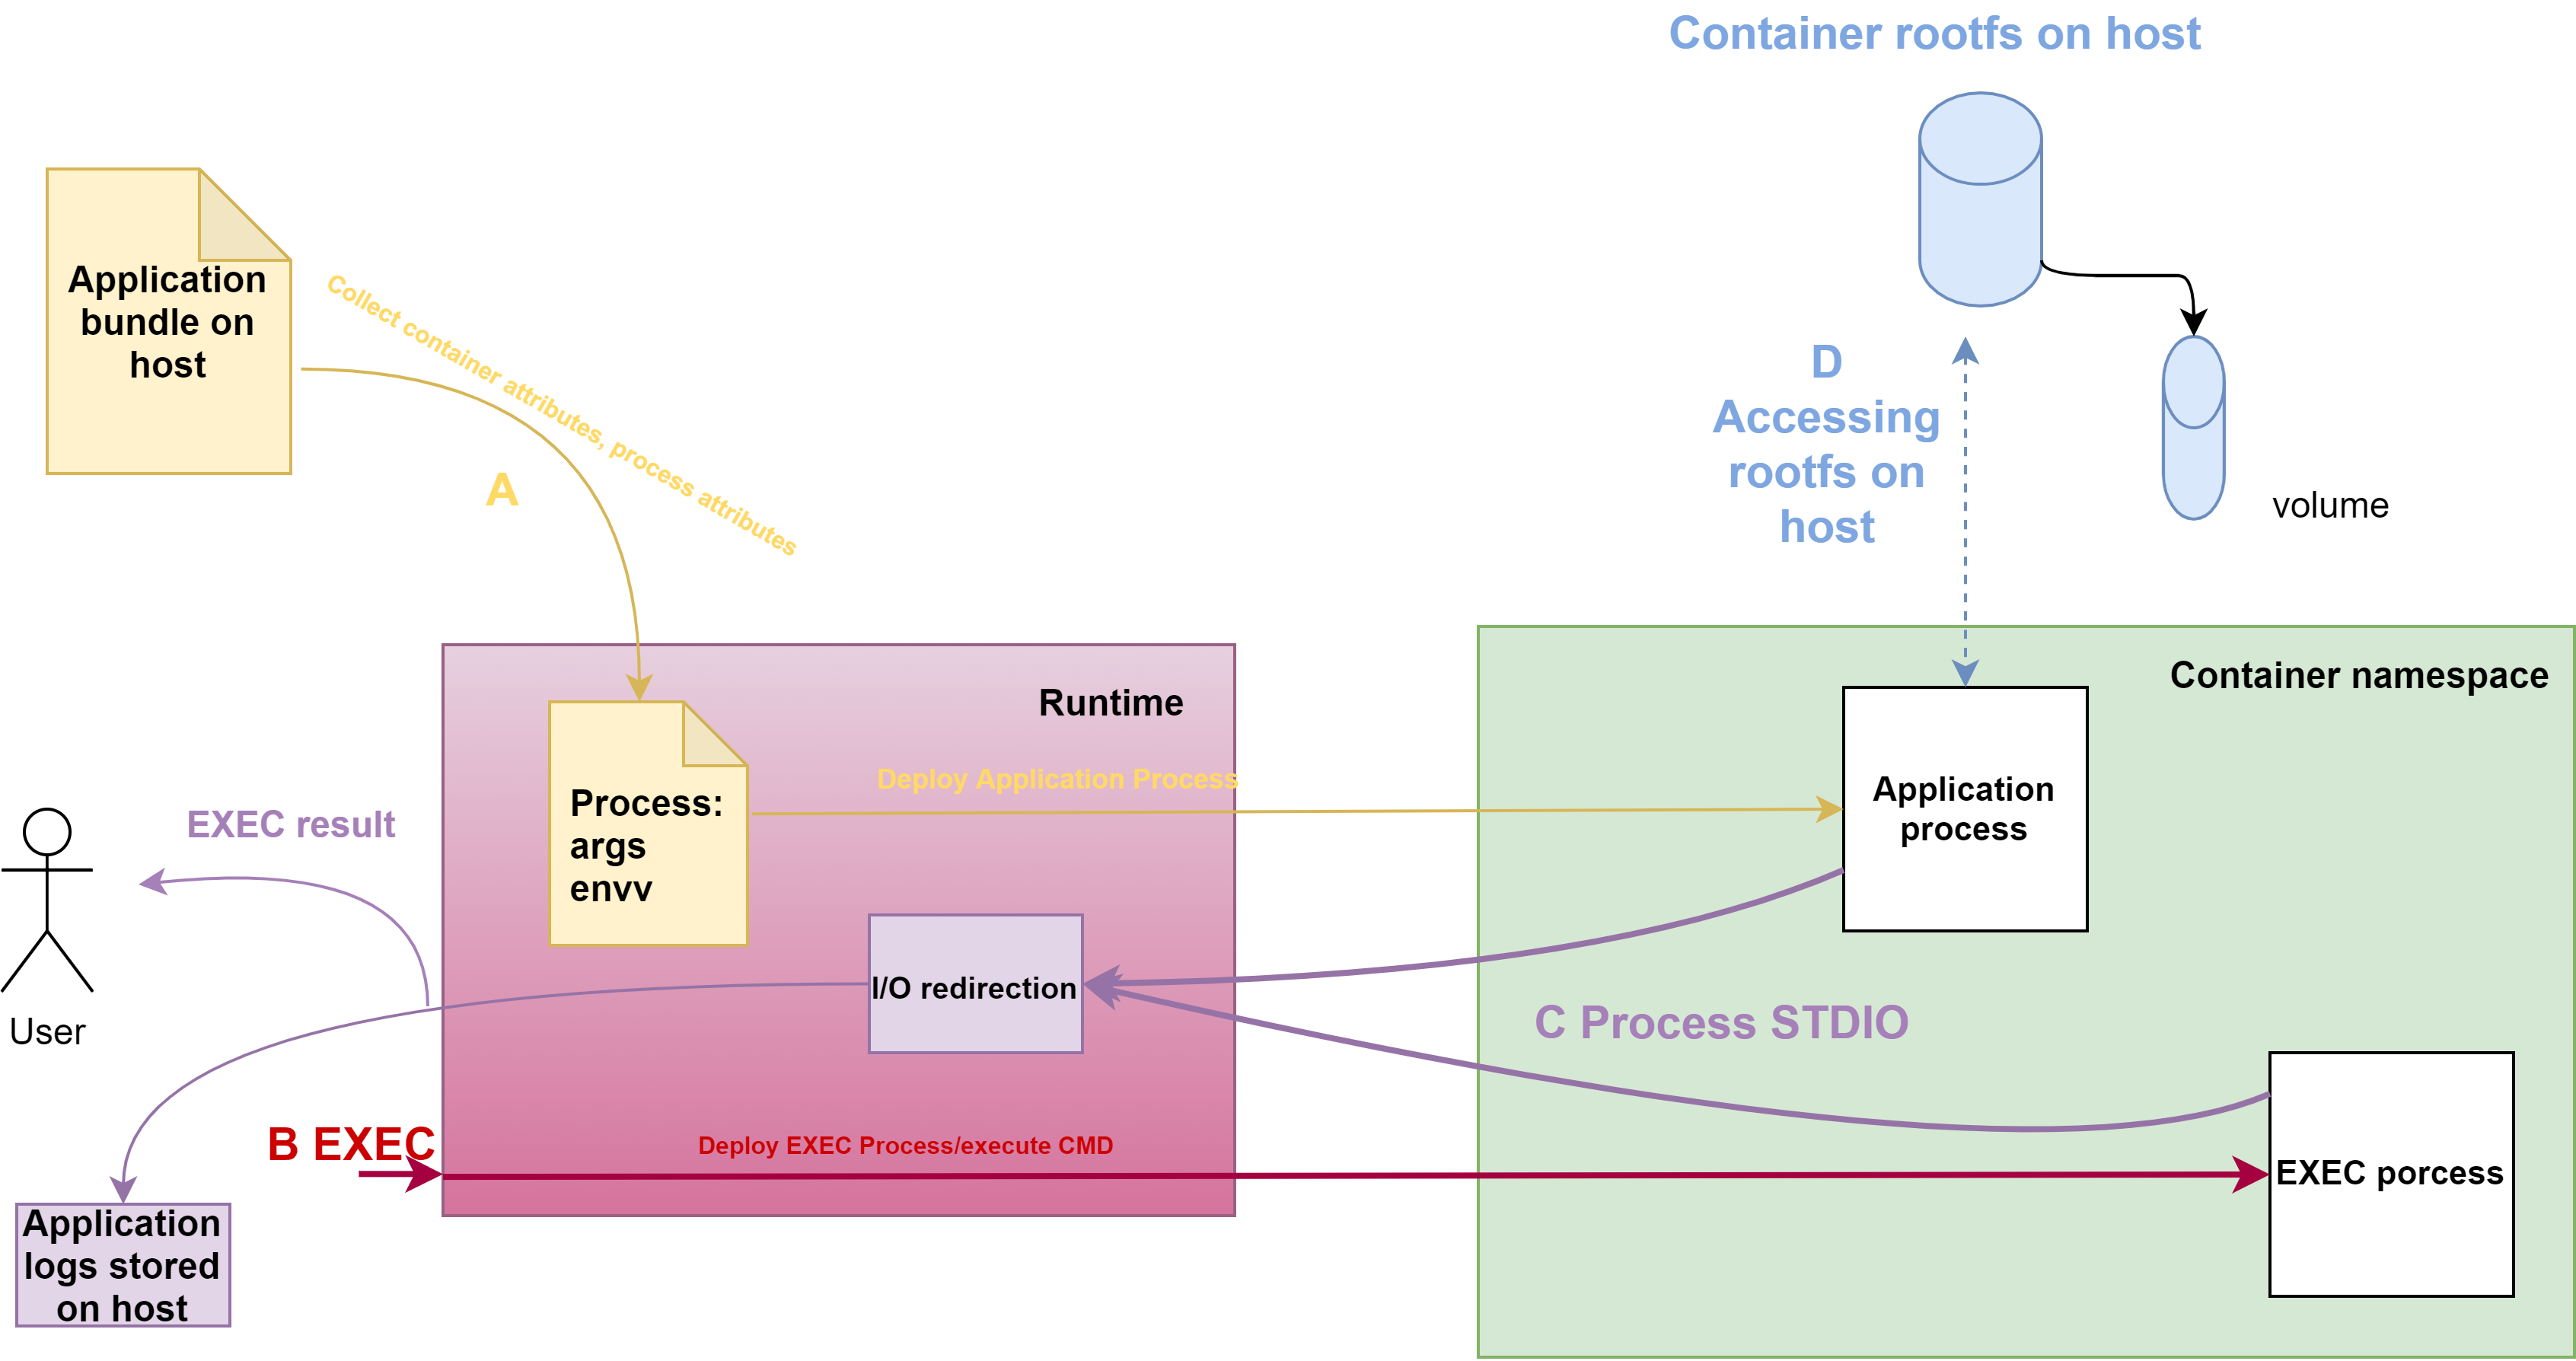
\includegraphics[width=0.8\textwidth]{images/security_analysis.png}
  \caption[Overview of the security analysis on OCI runtime interface]{Overview of the security analysis on OCI runtime interface}
  \label{fig:security_analysis}
\end{figure}


\subsection{Secret Deployment of Applications}
The application secrets deployment process defined in the OCI runtime interface can potentially result in secret disclosure. In confidential computing, there are three ways to inject secrets into an application: command line arguments, mounted files, and environment variables. According to the semantics of the OCI runtime interface, shim implements the operation 
\emph{create <container-id> <path-to-bundle>} for container creation. The \emph{<path-to-bundle>} points to an application bundle located on the host. As discussed in Section~\ref{sec:back_oci_runtime_spec}, this bundle, generated by a higher-level container runtime like Containerd~\cite*{containerd}, contains the necessary metadata for creating an 
application process and the application secrets. As shown in Part A of Figure~\ref{fig:security_analysis}, the shim will create the application process and deploy the secrets based on this application bundle. However, storing secrets on an untrusted host and relying on the shim for deployment is not a secure approach. An adversary with access 
to the host can manipulate these secrets. This compromises the confidentiality and integrity of the application secrets. Therefore, a new way of managing and deploying application secrets must be found. A reference solution can be found in Section~\ref{sec:design_Quark_Attestation_and_Provisioning_Infrastructure}.

\subsection{EXEC Operation}
\label{sec:Security_OCI_EXEC}

As depicted in Part B of Figure~\ref{fig:security_analysis}, shim's EXEC endpoint allows Anyone to issue commands to the applications. These include commands that allocate terminals, such as \emph{/bin/sh}, and others, like \emph{cat}, etc. Unfortunately, the container namespace does not implement authentication and access control mechanisms for EXEC requests from 
the shim. Therefore, an adversary can issue arbitrary commands to an application to collect its secret. For example, using \emph{printenv} to obtain the application's environment variable type secrets. Besides, the commands issued by the application owner may contain confidential data but are unprotected during transmission. As shown in Part B of Figure~\ref{fig:security_analysis}, the untrusted 
shim redirected commands and other metadata within the EXEC request to the container namespace. Consequently, the confidentiality and integrity of these commands may be compromised during transmission. To this end, the OCI interface~\cite*{oci-runtime-spec} should apply end-to-end cryptographic protection for these commands and add a checkpoint within the 
container namespace for authentication and access control on the EXEC requests. Any unauthorized commands should be denied. For further details, please refer to Section~\ref{sec:design_EXEC_Requests}.


\subsection{STDIO of Process}
\label{sec:security_analyse_STDIO_oci}
The OCI specification~\cite*{oci-runtime-spec} does not include cryptographic protection for the STDIN, STDOUT, and STDERR  of interactive processes and the STDOUT and STDERR of non-interactive processes. According to the OCI runtime interface semantics, there may be application processes or EXEC processes in the container's namespace. As depicted in Part C of 
Figure~\ref{fig:security_analysis}, the STDIOs of these processes are redirected by the shim. For application processes, the stream outputs of STDOUT and STDERR are stored as container logs on the host. For the EXEC process, command execution results are returned to the user via STDOUT or STDERR. In confidential computing, the application logs, command execution 
results, and data the application owner sends to interactive processes via STDIN may contain sensitive information. Hence, forwarding these data by the untrusted shim would jeopardize the data's confidentiality and integrity. As such, it is essential to ensure cryptographic protection for the STDIN, STDOUT, and STDERR of interactive processes, as well as 
the STDOUT and STDERR of non-interactive processes. A reference design can be found in Section~\ref{sec:design_prptect_privileged_request}

\subsection{Container Root Filesystem and Volume}

The OCI runtime interface~\cite*{oci-runtime-spec} lacks a mechanism to ensure the confidentiality and integrity of data in the container root filesystem and volumes. It does not define how the container root filesystem and volumes should be configured. Therefore, different runtimes can configure them as they see fit. For instance, virtual machine-based container 
runtimes (e.g., Kata runtimes~\cite*{Kata-Containers}) may mount the container root filesystem and volumes on the host and make them accessible to containers using a para-virtualized filesystem sharing mechanism (e.g., \emph{virtio-fs})~\cite*{kata_storage}. Alternatively, the runtime may treat the container root filesystem (comprising the container image layers) and volumes as block devices and expose them to the guest 
using \emph{virtio-block}~\cite*{kata_storage}. However, untrusted hosts can view or tamper with the data in these components (refer to part D in Figure~\ref{fig:security_analysis}). For example, viewing confidential data in volumes written by applications and tampering with binaries such as applications or shared libraries. Consequently, the confidentiality and 
integrity of container data are compromised. Note that according to the threat model in Section~\ref{sec:Threat_model}, filesystem protection is outside the scope of this thesis (i.e., protecting the data written to volumes and the filesystem). The threat model focuses on preserving the integrity of shared libraries and binaries, which include the application 
binary and the binaries loaded at application runtime (e.g., command binaries).


\subsection{System Call Interception}
\label{sec:security_analyse_oci_system_call}
The \emph{Seccomp} section of the OCI runtime specification~\cite*{oci-runtime-spec} outlines a method for restricting the system calls accessible to an application. This approach relay on the Linux kernel's feature \emph{Seccomp}~\cite*{seccomp} and a configuration file from the application bundle. During the creation of an application process, the runtime 
utilizes the file to configure \emph{Seccomp} accordingly. However, in confidential computing, the runtime is not trustworthy. It can tamper with the file to allow applications to execute system calls vulnerable to attack. Additionally, the host kernel is also deemed untrustworthy in this context. If the runtime were to rely on the \emph{Seccomp} mechanism 
within the host kernel, the system call interception would become meaningless. Thus, the OCI runtime specification must introduce a new mechanism for intercepting system calls. For further details, please refer to the reference design available in Section~\ref{sec:design_Interceptor}.


\subsection{Special Case for VM containers}
\label{sec:security_analyse_oci_vm}
For a VM container, the OCI interface defines the configuration of the hypervisor, guest kernel, and image. For example, the paths to the hypervisor, guest kernel,  and image,  as well as the startup parameters passed to the guest kernel and hypervisor. In confidential computing, ensuring that the environment for hosting containers 
(i.e., container namespace) is properly configured is critical. In the case of a VM container,  this entails the integrity of the guest kernel, and the guest kernel's startup parameters must be verifiable and protected. Besides, as the logs of the VM can potentially include confidential information, it becomes crucial to configure 
the VM logging system appropriately. To address these concerns, the OCI interface must define a remote attestation mechanism that enables the secret owner to validate that the VM is correctly configured.



\subsection{Summary}
\label{sec:security_analyse_oci_summary}
This section analyzes vulnerabilities in the OCI interface for confidential computing. These vulnerabilities include:
 \begin{enumerate}
  \item\label{vulnerability:1} Application secrets are deployed by untrusted runtime.
  \item\label{vulnerabilities:2} Processes' STDIOs lack cryptographic protection, i.e., protecting interactive processes STDIN, STDOUT, and STDERR, and non-interactive processes STDOUT and STDERR
      % \begin{enumerate}
      %     \item\label{vulnerabilities:2} Interactive processes STDIN, STDOUT, and STDERR lack cryptographic protection.
      %     \item\label{vulnerabilities:3} Non-interactive processes STDOUT and STDERR lack cryptographic protection.
      % \end{enumerate}
  \item\label{vulnerabilities:4}Lack authentication and access control over EXEC request
      % \begin{enumerate}
      %   \item\label{vulnerabilities:4} Anyone can issue commands to an application.
      %   \item\label{vulnerabilities:5} Commands issued by the application owner may contain confidential data but are not protected in transit.
      % \end{enumerate}
  \item Container root file system and volume
      \begin{enumerate}
        \item\label{vulnerabilities:5} Data written by the application to the root file system and volumes are accessible by untrusted entities on the host (out of the scope).
        \item\label{vulnerabilities:6} Binaries and shared libraries are vulnerable to tampering.
        % \item\label{vulnerabilities:8} Shared library files are vulnerable to tampering.
        % \item\label{vulnerabilities:9} Binary files loaded by the application during runtime are vulnerable to tampering.
      \end{enumerate}
  \item\label{vulnerabilities:7} The system call interception mechanism provided by Seccomp does not apply to confidential computing.
  \item\label{vulnerabilities:8} Lacking a mechanism to ensure that the container runtime environment is configured correctly. For VM containers, this means:
      \begin{enumerate}
        \item\label{vulnerabilities:9} Ensure that the correct guest kernel is loaded.
        \item\label{vulnerabilities:10} Ensure that the guest kernel startup parameters are correct.
        \item\label{vulnerabilities:11} Ensure that the guest kernel logging system is configured properly.
      \end{enumerate}
\end{enumerate}


\section{Analysis for the OCI runtime implementation in Quark}
\label{sec:security_analyse_quark_analysis}
Section~\ref{sec:security_analyse_oci_summary} provides a summary of vulnerabilities in the OCI runtime specification. The subsequent analysis will evaluate the security of Quark runtime deployed in the Kubernetes environment based on these vulnerabilities. Note that Qlib serves only as a developmental concept, as its code becomes part of the guest kernel (Qkernel) 
and the hypervisor (Qvisor) binaries through the compilation process. Henceforth, the Qkernel and Qvisor are used in the following to denote the guest kernel and hypervisor binaries, respectively. Furthermore, the term runtime defined in Section~\ref{sec:security_analyse_oci_analysis} represents the Quark shim and Qvisor, while the container namespace 
refers to the virtual machine encompassing both Qkernel and the application. Besides, the analysis uses \emph{Hcall::call id}, \emph{Qcall::call id}, and \emph{Ucall::call id} to specify a specific Hypercall, Qcall, and Ucall. Please consult Section~\ref{sec:Quark} for information on the Quark architecture and the workflow of Hypercall, Qcall, and Ucall.


\subsection{Application Secret Deployment Process in Quark}
\label{sec:security_analyse_secret_deployment}
\begin{figure}[htp]
    \centering
    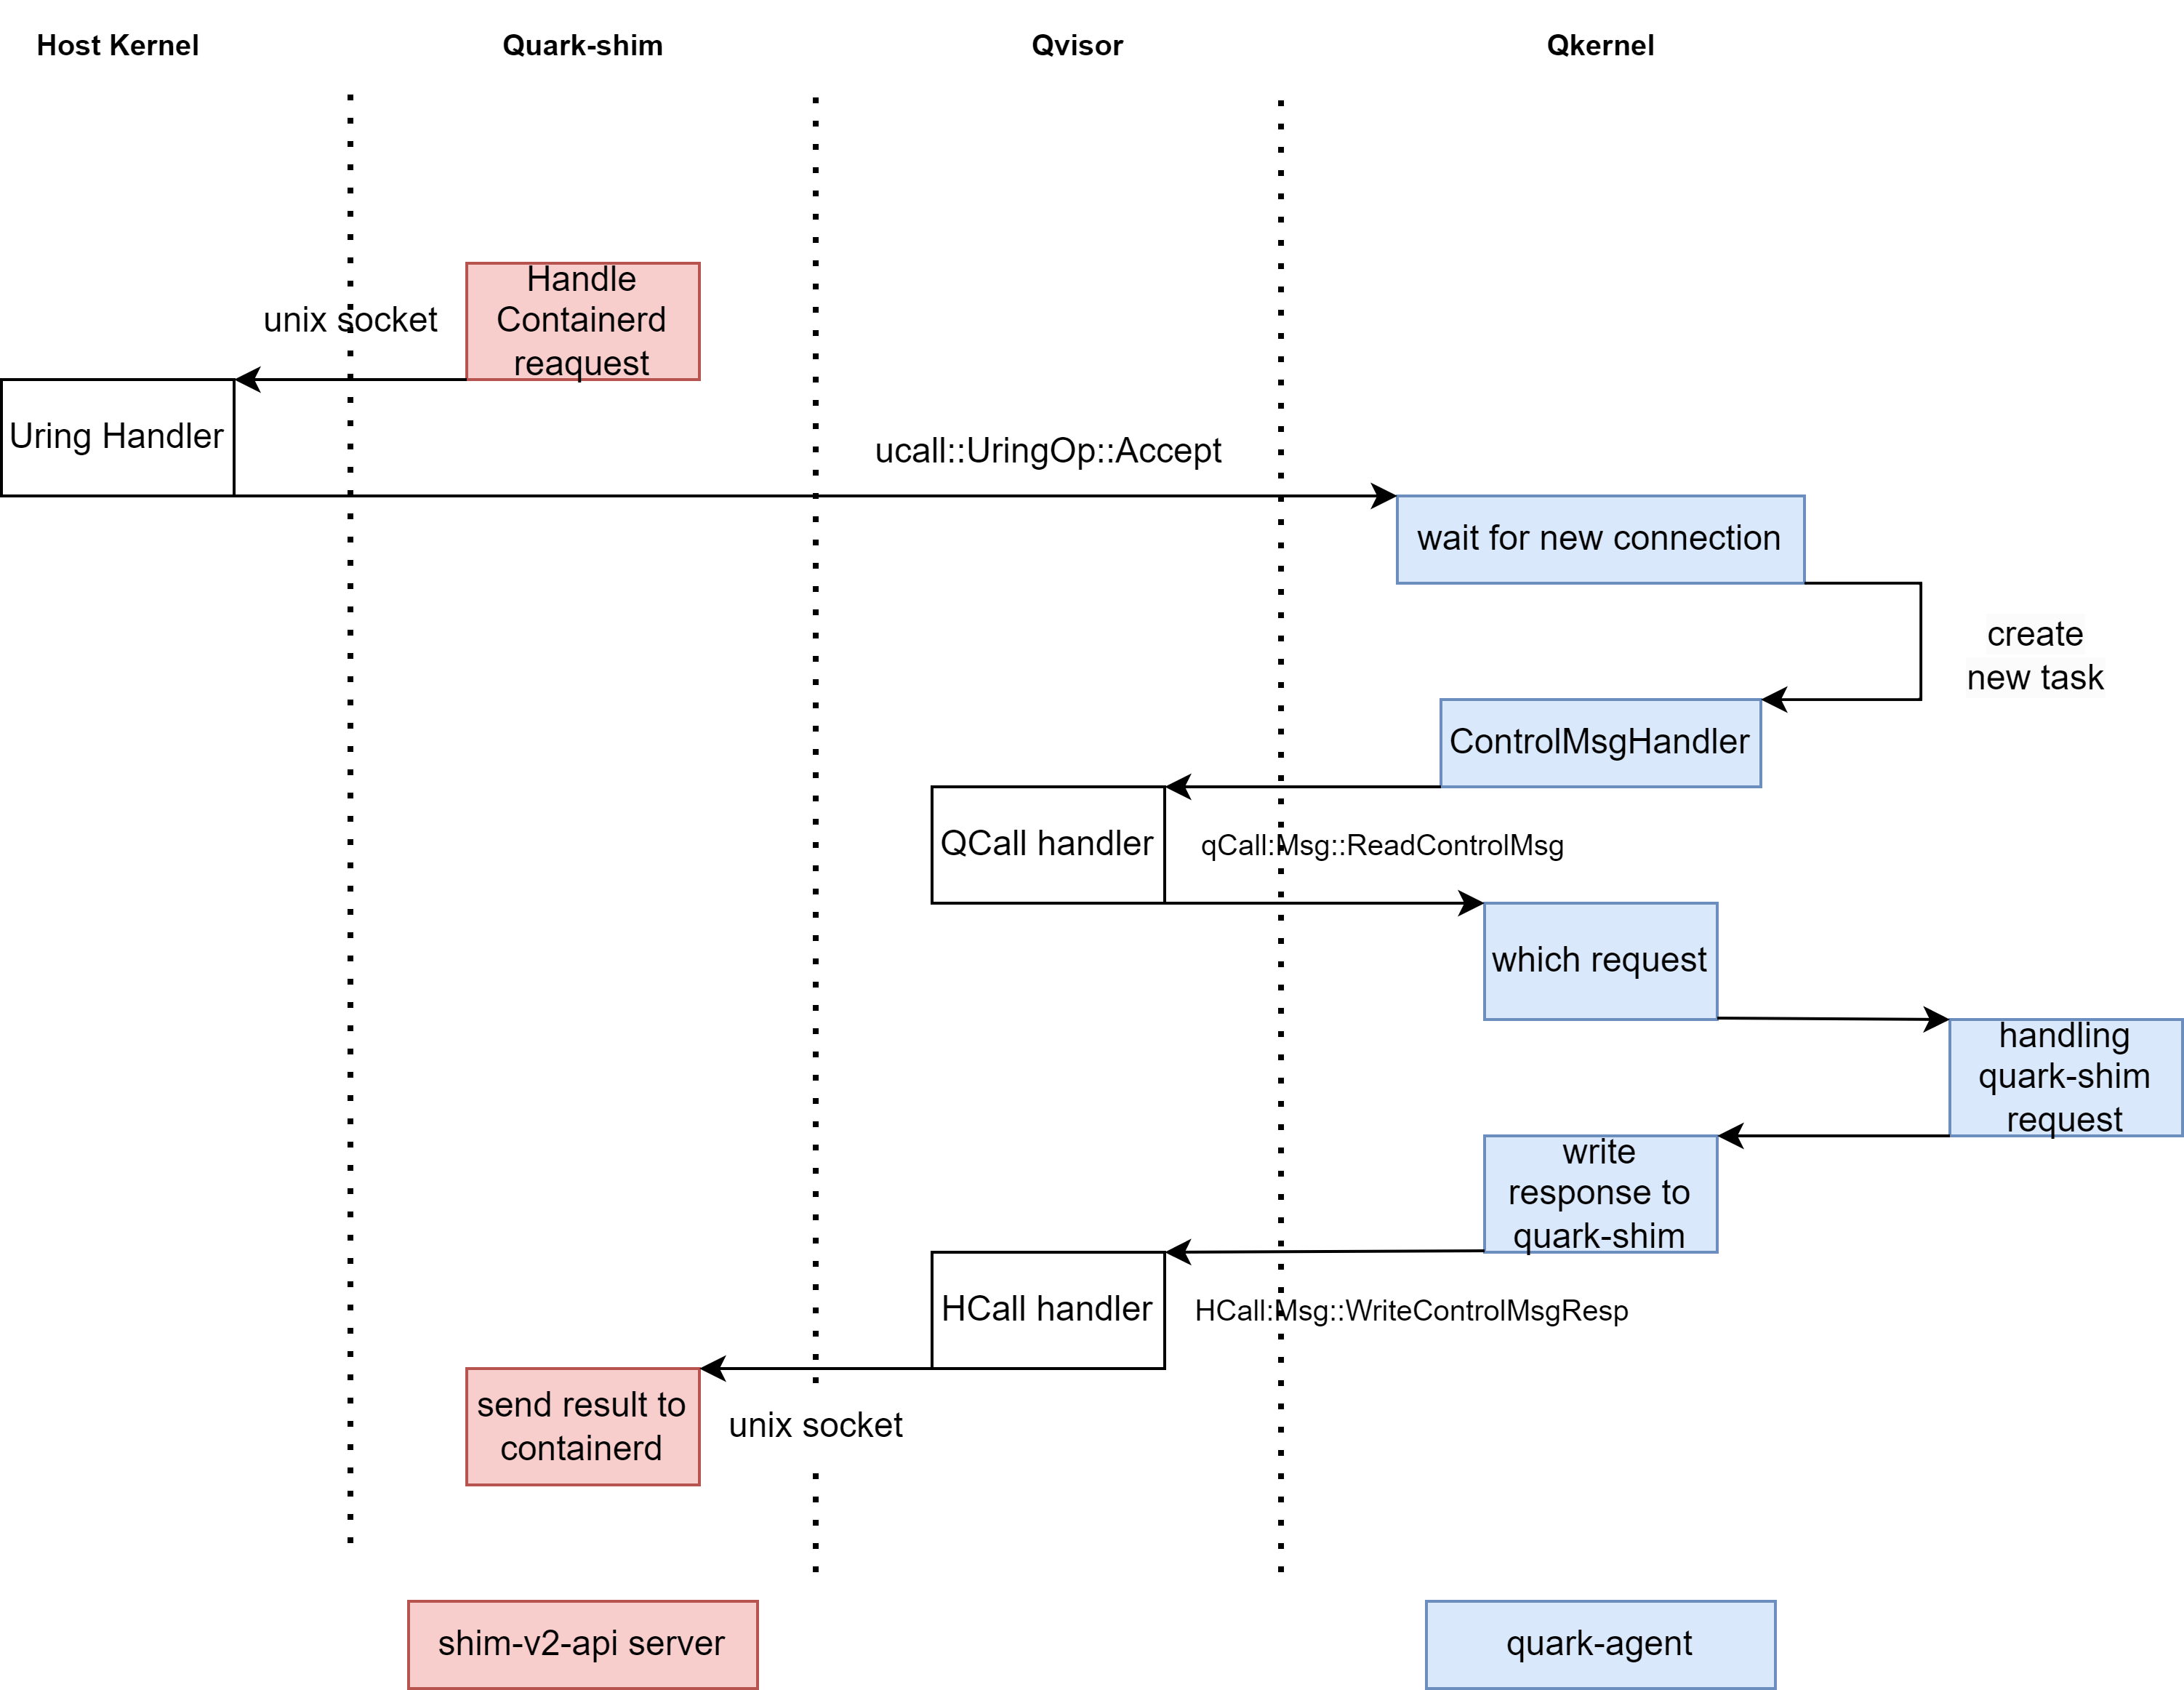
\includegraphics[width=0.8\textwidth]{images/quark-agent-work-flow.png}
    \caption[Quark Agent Workflow]{Quark agent workflow}
    \label{fig:quark_agent_work_flow}
\end{figure}


Untrusted Kubernetes~\cite*{k8s} and Quark shim manage and deploy application secrets, i.e., command line arguments, mount files, and environment variables. As shown in Figure~\ref{fig:quark_agent_work_flow}, when deploying the application, Containerd~\cite*{containerd} generates an application bundle and transmits it via the shim v2 API~\cite*{shim_v2} to the shim-v2-API server in the Quark shim. 
As discussed in Section~\ref{sec:back_oci_runtime_spec}, this bundle contains the rootfs of the application along with an OCI-compatible configuration file. Quark shim creates the root filesystem for the container on the host side, mounts the file type secret, and passes the process specification via the Unix socket. The specification contains metadata for creating a process in the guest, including command line 
arguments, environment variables, the type of STDIO (interactive or non-interactive IO), and the host file descriptor for transmitting data from/to the process STDIO. Upon receiving the specification, the Quark agent in the Qkernel will create an application process accordingly.


Quark-agent operates as a socket server accepting connection requests from the Quark Shim through \emph{Ucall::Uringop::accept()}. These requests include creating and deleting application processes, creating an exec process, etc. Upon receiving a request from Quark Shim to create an application or EXEC process, the Uringop::accept returns a host file descriptor 
that contains the process specification. As the agent in the Qkernel cannot read its contents directly, it employs \emph{Qcall::Msg::ReadControlMsg} to request the Qvivor to read the file descriptor and return the specification. Based on the specification, Quark-agent creates a guest user process. Specifically, the command line arguments and the environment variables 
are pushed to the process stack, and the STDIO of the process is set accordingly to the type of STDIO specified in the specification. Further details about the process's STDIO can be found in section~\ref{sec:security_analyse_STDIO}.


Using Kubernetes~\cite*{k8s} to manage application secrets and deploying them through untrusted Containerd~\cite*{containerd} and Quark shim lead to secret disclosure. Specifically, individuals with cluster access can exploit the kubectl tool to manipulate secrets. Furthermore, the Containerd and Quark Shim can tamper with these secrets during the application deployment. Besides, 
when Quark-agent uses the Qcall interface to request Qvisor to read the process specification, Qvisor could potentially steal or modify these secrets.  The aforementioned analysis aligns with vulnerability~\ref{{vulnerability:1}} found in the analysis of the OCI runtime interface. For this reason, the management and deployment of secrets must be offloaded from Kubernetes, Quark Shim, 
and Qvisor. A detailed explanation of the mitigation can be found in section~\ref{sec:design_Quark_Attestation_and_Provisioning_Infrastructure}.


\subsection{Guest User Space Process STDIO}
\label{sec:security_analyse_STDIO}

The Quark agent loads the corresponding binary and initiates a guest user-space process for handling the request, such as creating an application or executing a command. Thus, Quark handles the application process STDIO in the same way as it handles the exec process STDIO. For instance, when Containerd~\cite*{containerd} wishes to create an EXEC process in Qkernel, 
three named pipes are created for the process's standard input, output, and error. These are then passed to Quark Shim with other metadata. Quark Shim then employs these data to create the EXEC request's process specification. The Quark handles the process's STDIO differently based on the terminal keyword in the process specification.


\begin{figure}[ht] 
    \begin{subfigure}[b]{0.5\linewidth}
      \centering
      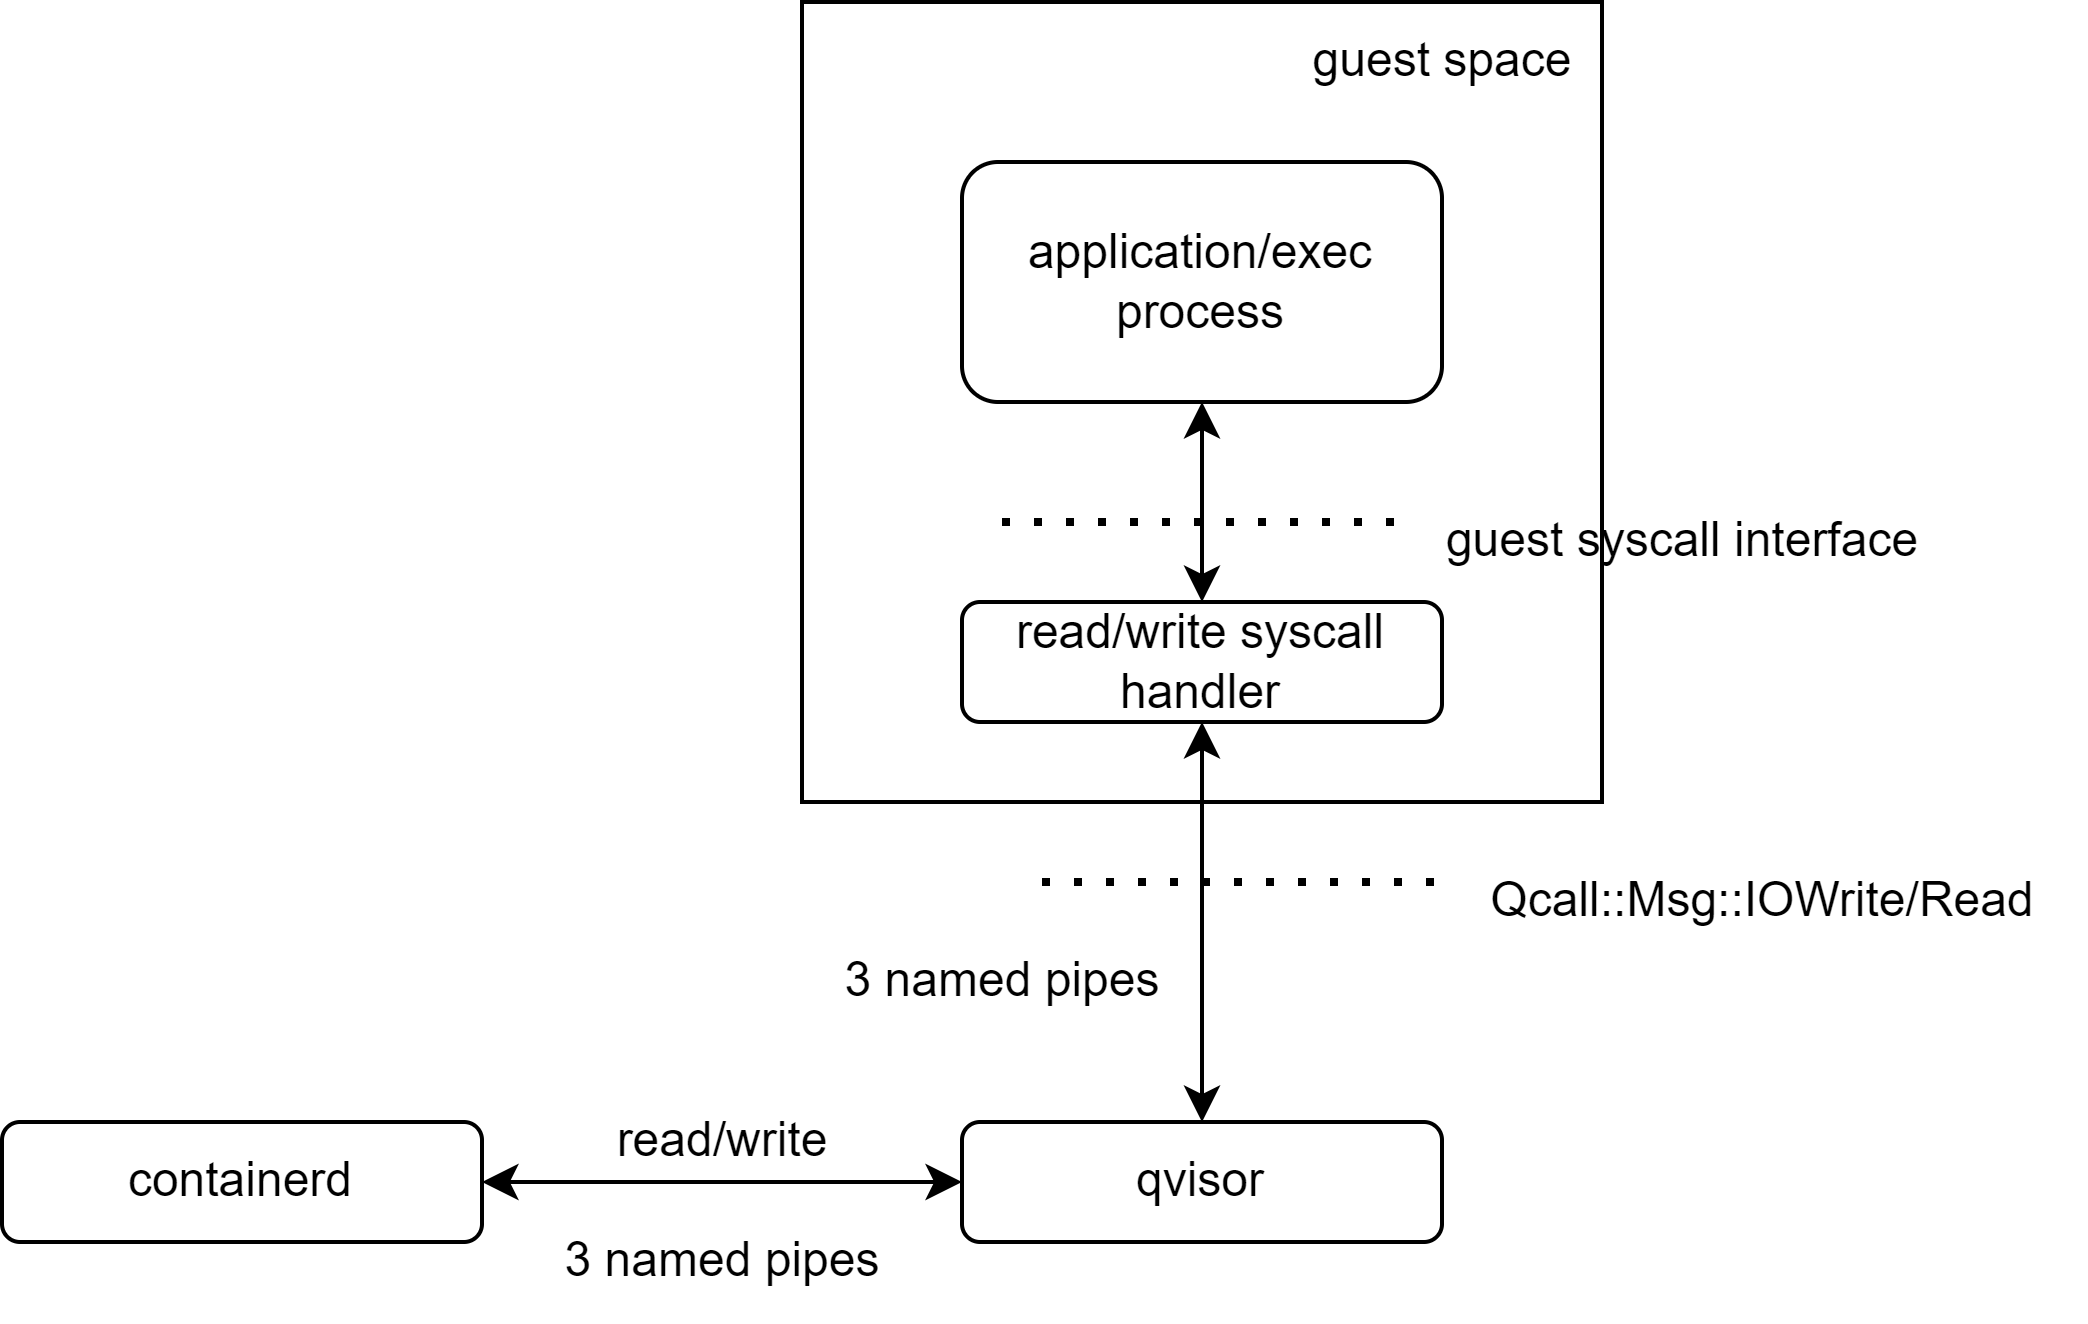
\includegraphics[width=0.9\linewidth]{images/normorl_io.png} 
      \caption{Normal IO} 
      \label{fig1:a} 
      \vspace{4ex}
    \end{subfigure}%% 
    \begin{subfigure}[b]{0.5\linewidth}
      \centering
      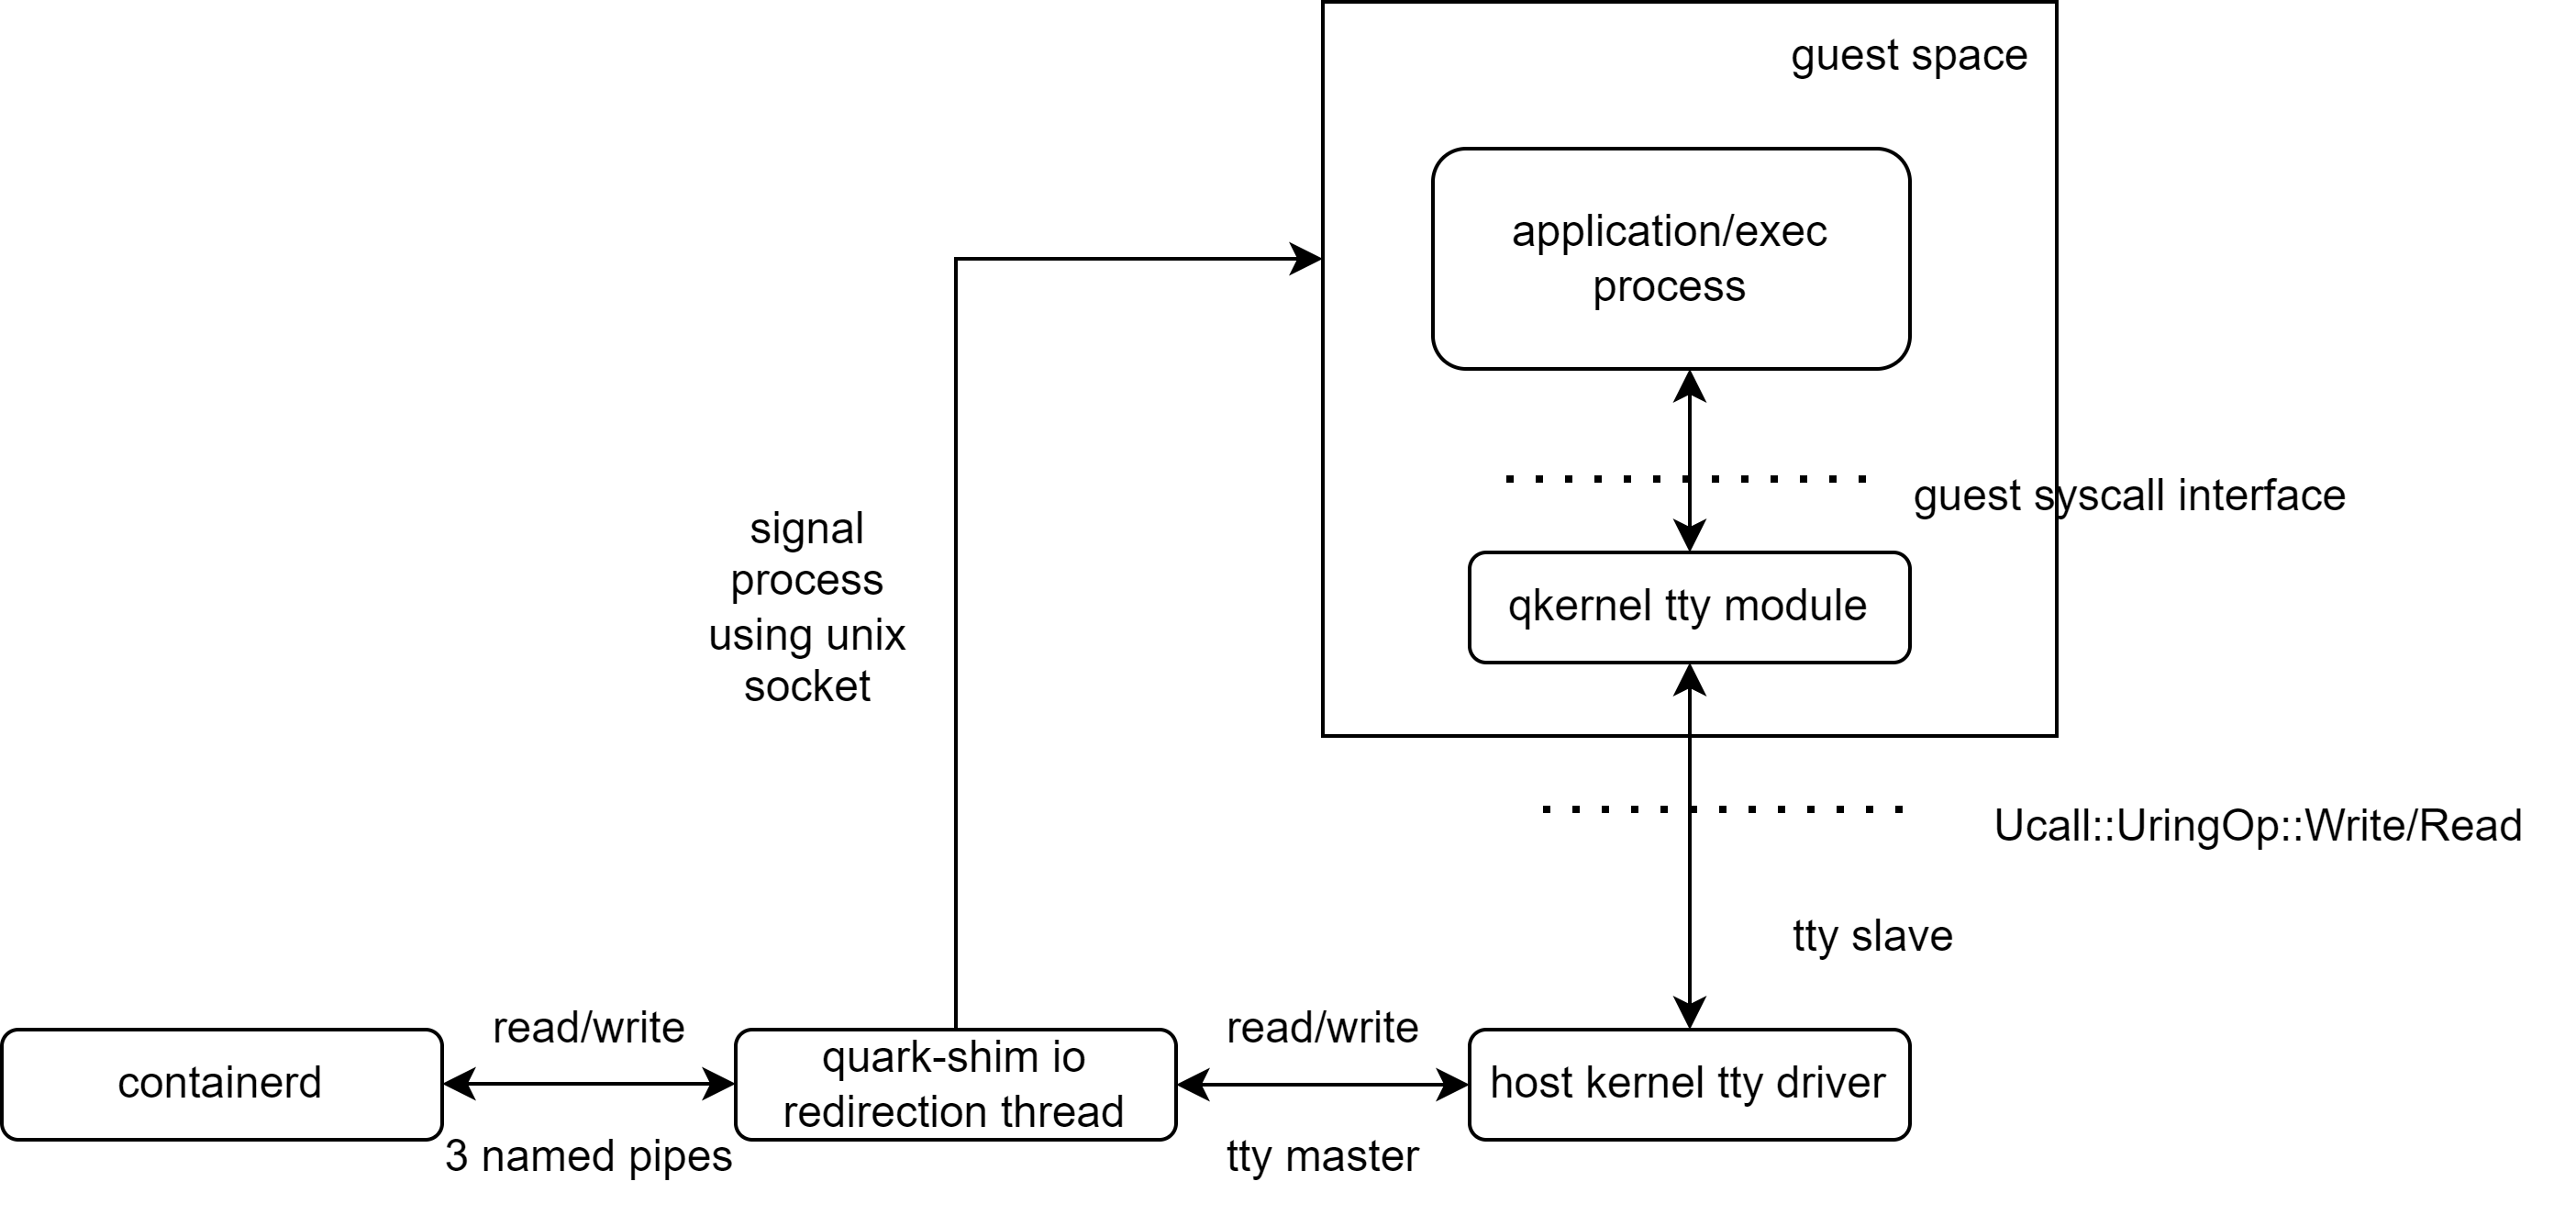
\includegraphics[width=0.9\linewidth]{images/termianl_workflow.png} 
      \caption{Terminal IO} 
      \label{fig1:b} 
      \vspace{4ex}
    \end{subfigure} 
    \caption{Guest User Space Process STDIO Handling Workflow}
    \label{fig1} 
\end{figure}


The terminal keyword is true for an interactive process. In this case, as illustrated in Figure~\ref{fig1} (b), Quark Shim creates an asynchronous terminal IO redirection thread and requests a TTY pair from the host kernel (TTY master and TTY slave). The TTY slave is then sent to the Quark agent, where it is set as STDIN, STDOUT, and STDERR of the process. 
The Qkernel TTY module can read and write the TTY slave through the UCLL interface. Furthermore, the redirection thread filters the signals in the STDIN-named pipe and transfers the data between the TTY master and the named pipes. The filtered signals include SIGINT, SIGQUIT, and SIGTSTP, which are forwarded to the Quark agent via the Unix socket. In this case, 
the Quark agent will signal the process accordingly. For instance, when the character \textasciicircum C (ASCII code 3) appears in the STDIN-named pipe, the redirection thread sends SIGINT to the process, ultimately terminating it. Besides, the data written to the TTY master and slave are processed by the host kernel TTY drive. For data written to the slave, the driver translates 
each line feed (\textbackslash n) into a carriage return followed by a line feed (\textbackslash r\textbackslash n). This editing is required because the user-side terminal needs these two characters to start a new line of text. Also, for characters written to the TTY master, the driver first echoes them back to the user and stores a copy in an internal buffer. 
When the user presses the enter key (\textbackslash r), it copies the buffered data to the TTY slave. As such, the terminal will not work without the host kernel TTY driver.

 

The terminal keyword is false for a non-interactive process. In this case, as shown in Figure 4.2a, Quark Shim directly sends the three named pipes to the Quark agent. It then creates the process and uses the pipes as STDIN, STDOUT, and STDERR. Unlike the former case, Qkernel uses the Qcall interface for STDIO data transmission.

While the process is running, Containerd~\cite*{containerd} will keep the three named pipes open. For the application process, STDOUT and STDERR stream output is saved as container logs to a location specified by Kubernetes~\cite*{k8s}. For an EXEC process, the command execution result is returned to the user via STDOUT or STDERR.


The above description shows that untrusted entities (such as Quark shim, Qvisor, and Containerd) are responsible for processing the STDIO data streams of both interactive and non-interactive processes. Consequently, these entities can steal privacy-sensitive data within the processes' STDIO data streams. This finding aligns consistently with the 
analysis presented in Section~\ref{sec:security_analyse_STDIO_oci}. Therefore, the STDIO data stream of the guest process must be cryptographically protected. Further information can be found in Section~\ref{sec:design_STDIO_PROTECTION}.


\subsection{EXEC Operation}
As discussed in Subsection~\ref{sec:security_analyse_secret_deployment}, the Quark agent located in Qkernel is responsible for handling the EXEC request from Quark shim. However, it lacks authentication and access control over these requests. Thus, an attacker can issue arbitrary commands to the application to collect its secrets. Moreover, the commands are 
redirected to Qkernel by Containerd~\cite*{containerd} and Quark shim, along with other metadata in EXEC request. Specifically, when Quark shim receives an EXEC request from Containerd, it generates a process specification from the metadata received from Containerd. This specification includes the command and its parameter, the STDIO type, the environment 
variables, etc. Subsequently, Quark Shim forwards this specification to the Quark agent via a Unix socket, wherein a guest process is created to execute the command (Figure~\ref{fig:quark_agent_work_flow}). Since the commands issued by the application owner may contain confidential data. Forwarding these commands by Containerd, Quark Shim poses potential risks 
to their confidentiality and integrity. This finding aligns with the analysis presented in Section~\ref{sec:Security_OCI_EXEC}. As such, end-to-end cryptographic protection for these commands should be adopted, and authentication and access control checkpoints should be added in Qkernel. By doing so, any unauthorized commands can be denied. For further information, 
please refer to section~\ref{sec:design_EXEC_Requests}.


\subsection{Container Root Filesystem and Volume}
Quark shim sets up the application's root filesystem on the host and enables applications to access the root filesystem through a para-virtualized file system sharing mechanism. For instance, when the application utilizes the guest-read system call to access a file, the Qkernel will request the host to read the target file via Hypercall or Ucall. As a result, the 
data that the application writes to its filesystem and volumes is visible to the host. In this scenario, the untrusted host can manipulate the confidential data stored in the filesystem. Therefore, Qkernel must implement a filesystem shield. However, this vulnerability is beyond the scope of this thesis, as defined by the threat model in 
Section~\ref{sec:Threat_model}.

This thesis aims to guarantee the integrity of binaries and shared libraries loaded from the host. Hence, the following two subsections analyze the security issues that occurred during the loading of binaries and shared libraries by Qkernel.

\begin{figure}[ht] 
  \begin{subfigure}[b]{0.5\linewidth}
    \centering
    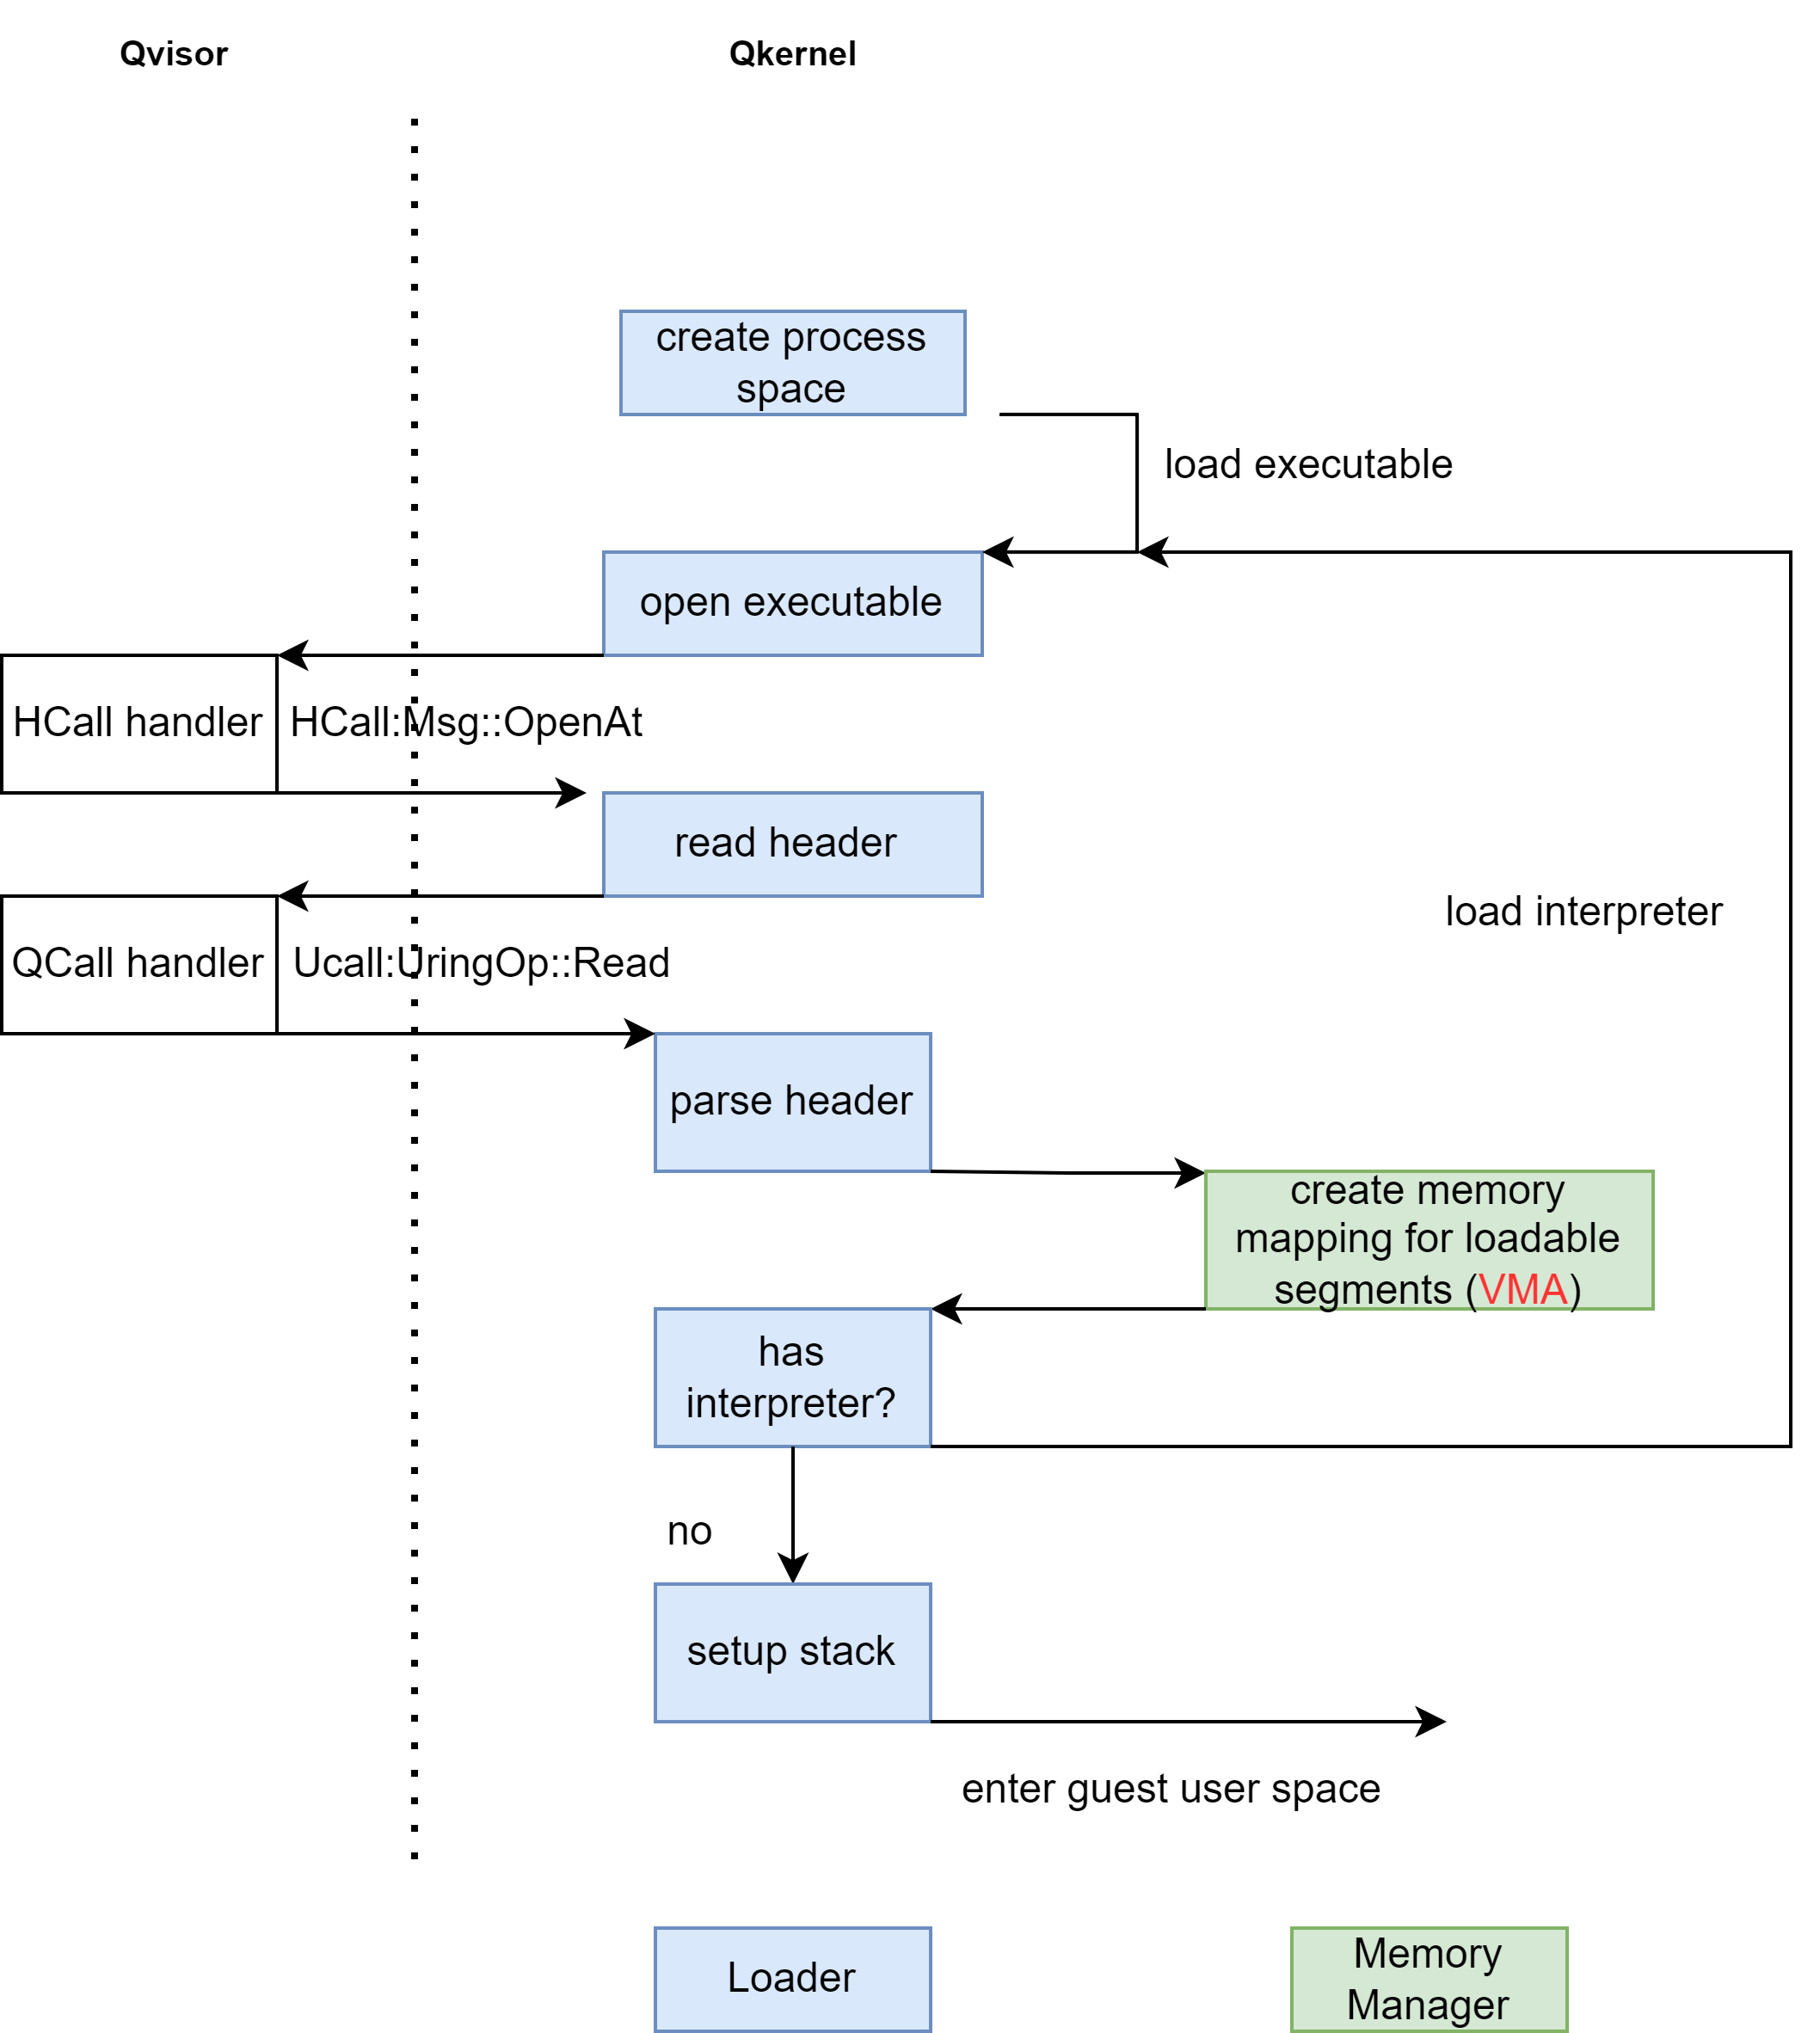
\includegraphics[width=0.9\linewidth]{images/loader_flow.png} 
    \caption{Loader setup memory mappings during application startup} 
    \label{fig2:a} 
    \vspace{4ex}
  \end{subfigure}%% 
  \begin{subfigure}[b]{0.5\linewidth}
    \centering
    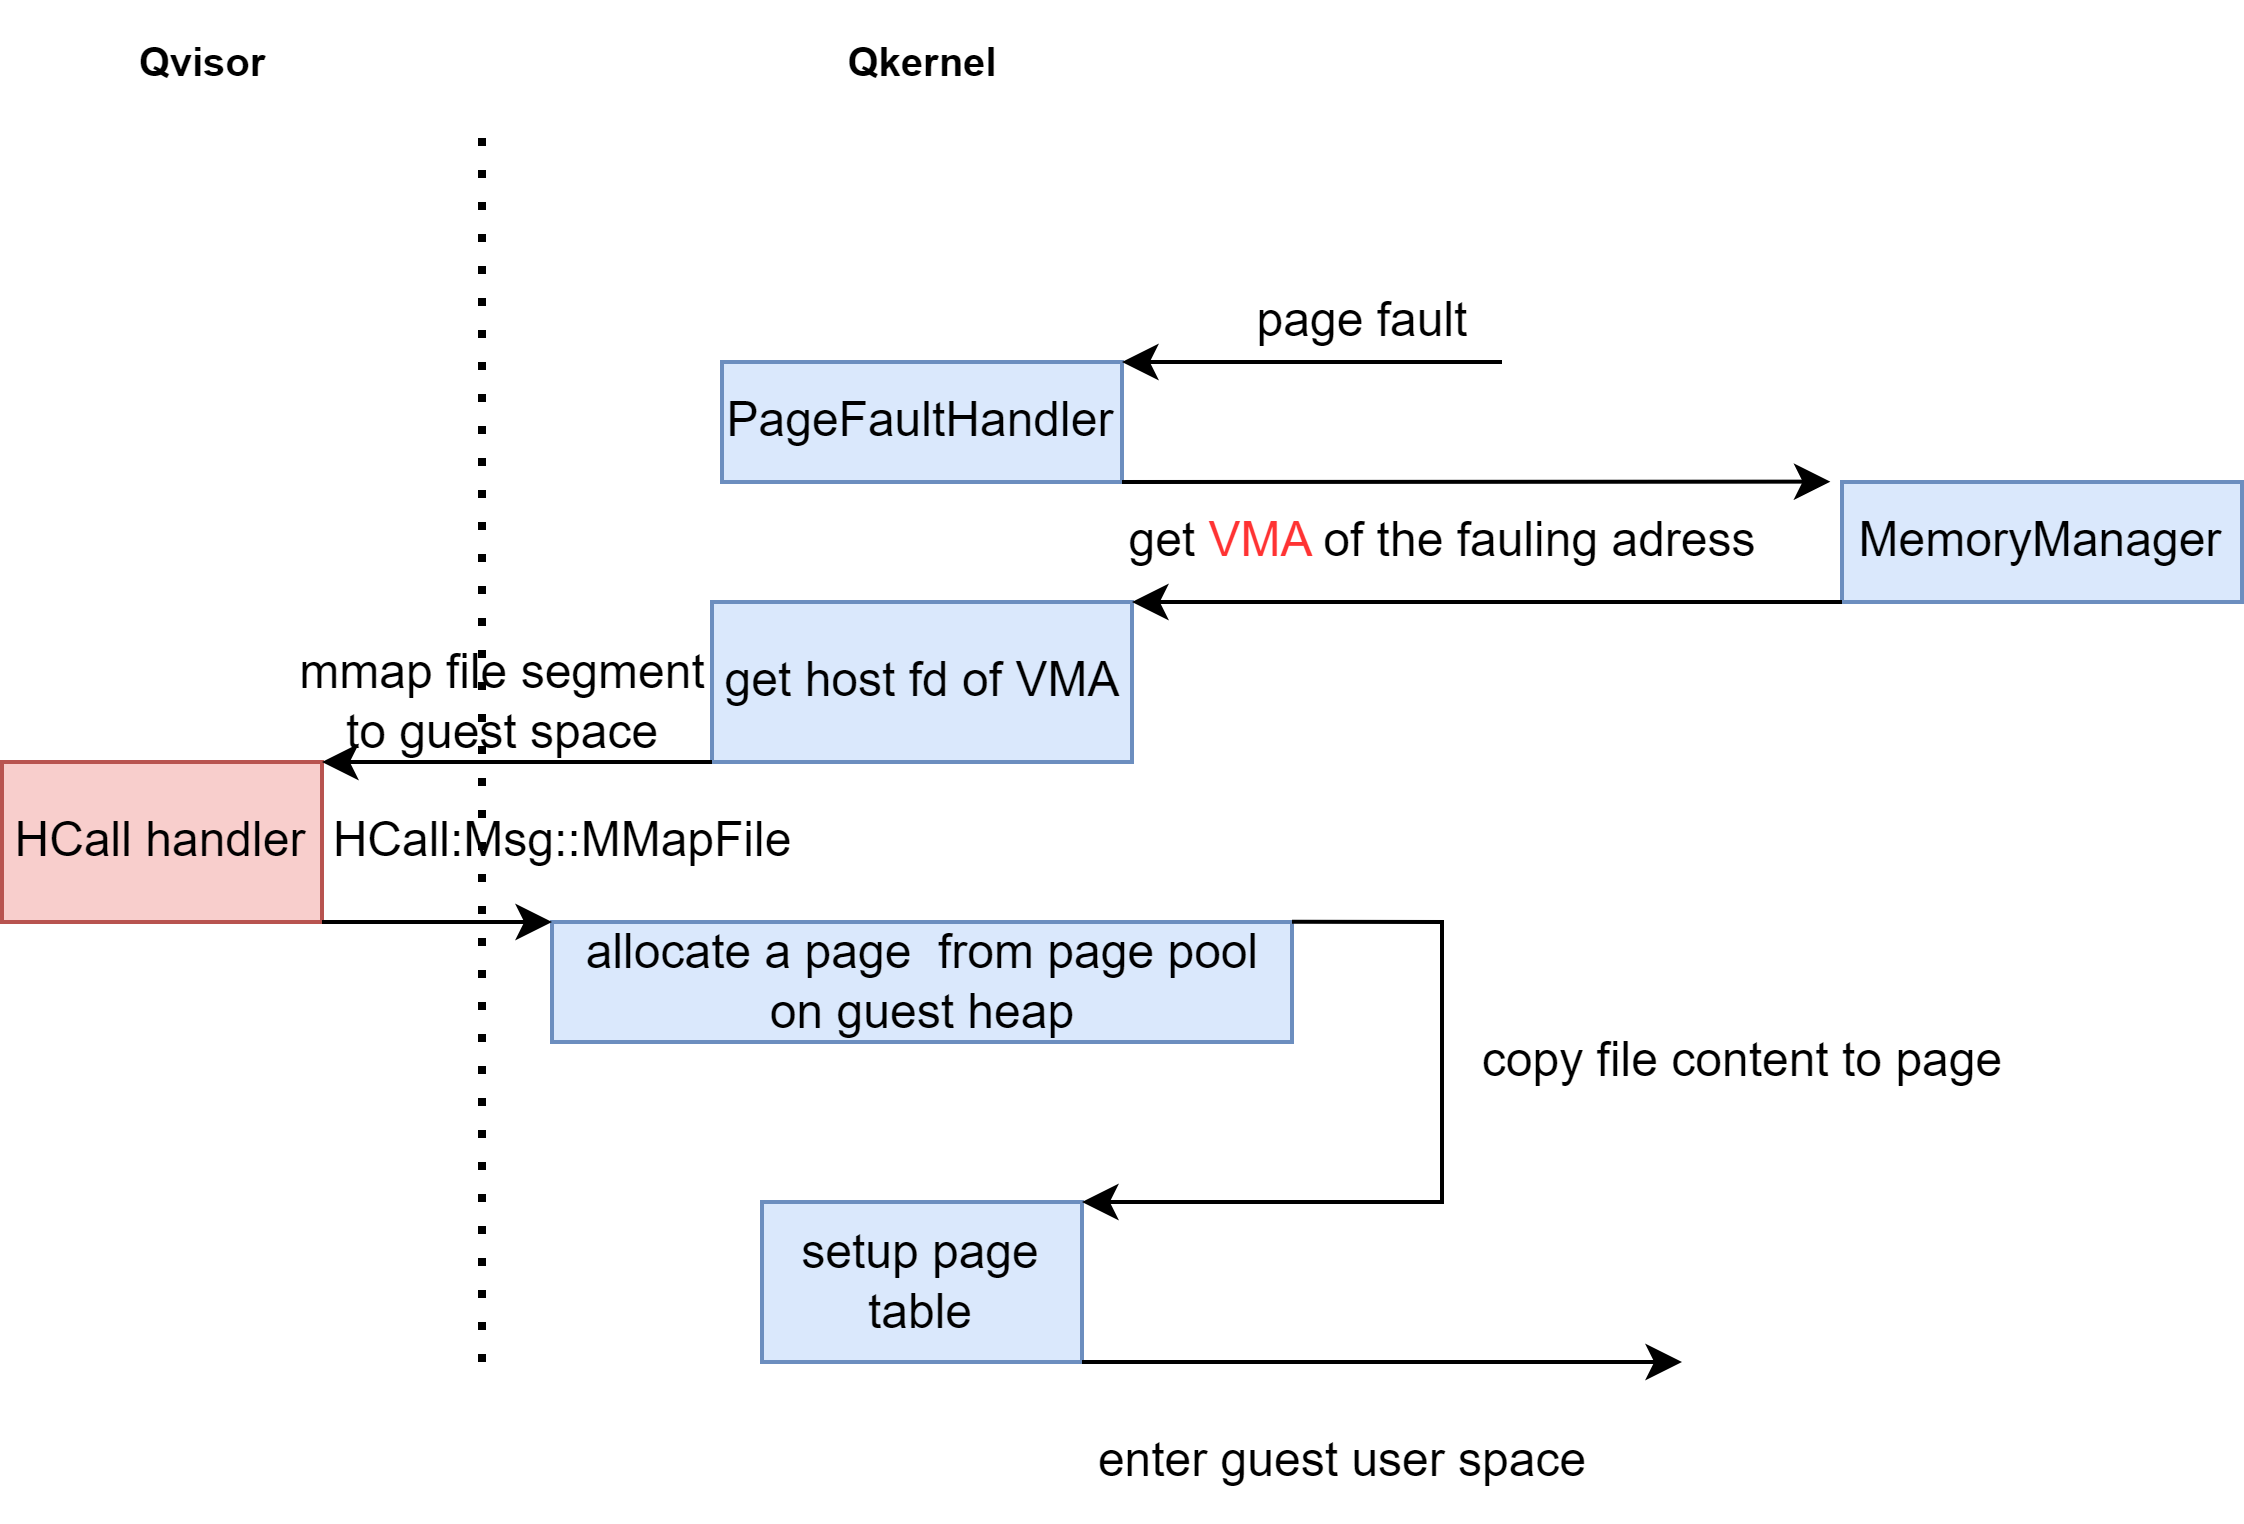
\includegraphics[width=0.9\linewidth]{images/page_fault_handling.png} 
    \caption{Page Fault Handling} 
    \label{fig2:b} 
    \vspace{4ex}
  \end{subfigure} 
  \caption{Application binary loading process}
  \label{fig2} 
\end{figure}

\subsubsection{Loading compromised Application Binary during Startup}
\label{sec:app_binary_loading}
The application binary is stored on the host. During the setup of the application process, the Qkernel loader opens the application binary using Hcall::Openat, reads its ELF header into the Qkernel using the \emph{Ucall::read}, and then requests the Qkernel virtual memory manager to create a private virtual 
memory area (\acrshort{VMA}) for each loadable segment defined in the ELF file (Figure~\ref{fig2} (a)). When the application process runs, accessing an address within the \acrshort{VMA} will trigger a page fault, which is handled by the Qkernel page fault handler.
 
The workflow for the page fault handling can be found in Figure~\ref{fig2} (b). Since the \acrshort{VMA} of a loadable segment is private, the page fault handler uses hcall::mmap to request Qvisor to map the loadable segment into a guest's physical address. It then allocates a page from the page pool on the Qkernel heap and copies the 
segment's contents from the guest's physical address to this page. Finally, a page table entry (guest virtual address -> address of the page) is created. After this, the page fault handler hand over the control to the guest user process.
 
Since the application binary is loaded from the host,  an attacker can induce Qkernel to execute compromised codes. For instance, the loader might request Qvisor to open binary A using \emph{Hcall::openat}. Nevertheless, instead, Qvisor provides the descriptor of file B. As a result, the loader creates the 
wrong memory mapping. Consequently, the page fault handler will load the code from file B instead of file A. Furthermore, since the page fault handler uses \emph{Hcall::mmap} to map the executable into the guest's physical space, an attacker could manipulate the Qvisor to map compromised code. In this case, 
the page fault handler copies this code to a page, creates a page table entry, and then returns to the application process without an integrity check.  
 
To this end, the application binary should be loaded to the guest and measured when the Qkernel loader creates the \acrshort{VMA}s for it. The measurements should be forwarded to relying party for integrity checking. Further detail can be found in Section~\ref{sec:Enclave_Runtime_Measurement}. 

\begin{figure}[htp]
  \centering
  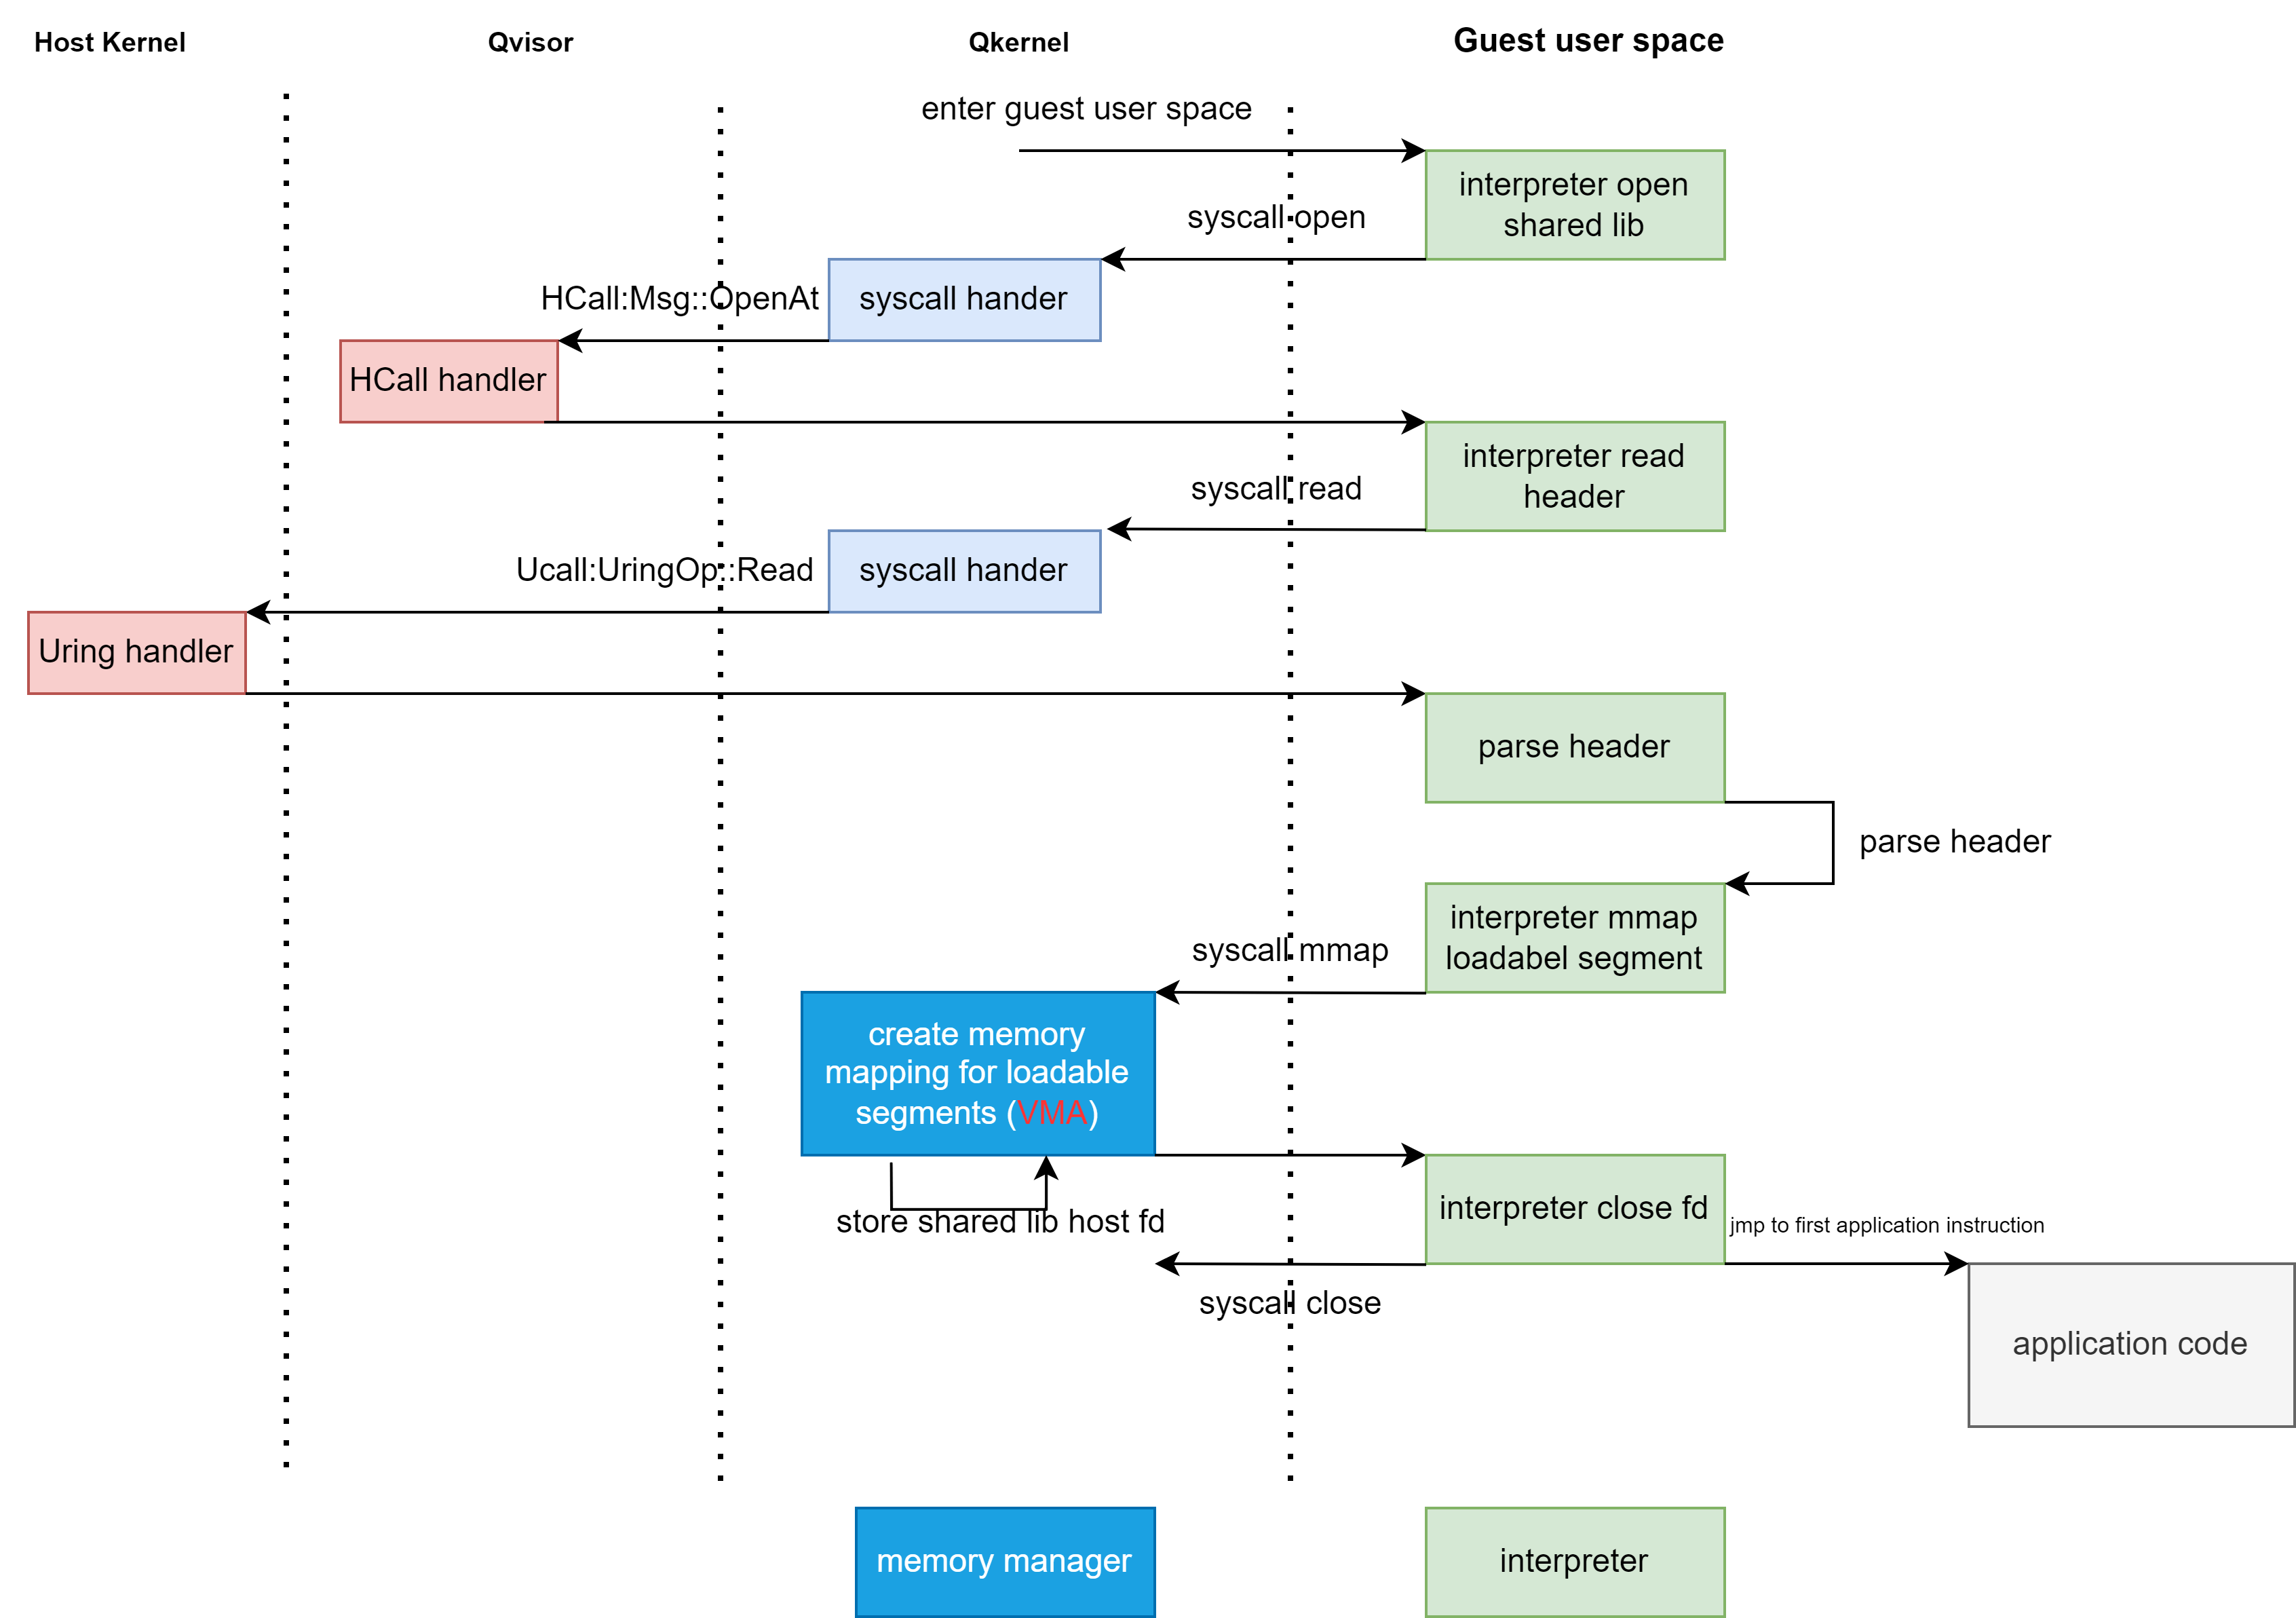
\includegraphics[width=0.6\textwidth]{images/load_shared_libarart.png}
  \caption[Interpreter setups shared library's memory mappings]{Interpreter setups shared library's memory mappings}
  \label{fig:load_shared_libarart}
\end{figure}


\subsubsection{Loading compromised Binary at Runtime}
Dynamic libraries are stored on the host and loaded at application runtime by the interpreter. When the application is a dynamically linked executable, the interpreter's code is executed upon launching the application process. As depicted in Figure~\ref{fig:load_shared_libarart}, the interpreter uses the \emph{open}, \emph{read}, and \emph{mmap} 
system calls to create private memory mappings (\acrshort{VMA}s) for the loadable segments in a shared library. Accessing an address within the \acrshort{VMA}s triggers page faults. The page fault handler handles the fault like how it handles page faults when accessing the \acrshort{VMA} of the application binary.
Since the process of how the Qkernel creates memory mapping and later loads code to the guest for shared libraries and application binary are very similar, the issues encountered in the previous section also apply here. 
 
Executing a command at runtime will cause the Qkernel to load the command binary. The binary loading mechanism has already been discussed in section~\ref{sec:app_binary_loading}. Therefore, a malicious user can inject malicious code into the Qkernel. 
 
Regarding the mitigation, Qkernel should measure the binaries and shared libraries after its \acrshort{VMA} is created and checks its correctness using the reference hashes in the policy file obtained from the relying party. Further detail can be found in Section~\ref{sec:Enclave_Runtime_Measurement}. 


% \subsubsection{Lack of Management of Application Restart}
% In an unexpected application crash, Kubernetes~\cite*{k8s} may recreate a pod to execute the crashed application or restart the program within the original pod if it still exists~\cite*{k8s}. In the latter case, Qkernel reloads the application binaries from the host and provides the application with the secret 
% obtained from relying party during the first startup. An attacker may use this opportunity to inject malicious code into Qkernel. To mitigate this threat, Qkernel should measure the application recreation process and compare the result with the initial 
% application startup measurement stored on guest memory. If the two hashes do not match, Qkernel should panic.  Further detail can be found in Section~\ref{sec:Enclave_Runtime_Measurement}. 

\subsection{No restriction to the available System Calls for Applications}

Quark does not implement the system call intercept (Seccomp~\cite*{seccomp}) as specified in the OCI runtime specification~\cite*{oci-runtime-spec}. Thus, vulnerable system calls can be exploited to launch attacks against both the Qkernel and other processes. For instance, an attacker could initiate a malicious EXEC process and manipulate it 
to utilize vulnerable system calls in order to steal application secrets. Furthermore, the discussion in Section~\ref{sec:security_analyse_oci_system_call} revealed that Seccomp is not an appropriate solution for confidential computing. Therefore, a novel mechanism for intercepting guest system calls is proposed in Section~\ref{sec:design_Interceptor}. This mechanism allows the 
application owner to specify the permissible system calls for the application while ensuring that the guest system call interceptor is properly configured. 




\subsection{VM Configuration}

As described in Section~\ref{sec:security_analyse_oci_vm}, the correct VM configuration involves loading the correct guest kernel binary and the startup parameters, as well as configuring the guest logging system properly. In the case of Quark, the Qkernel is the binary that Qvisor loads into the guest's memory during the VM setup process. However, 
since the untrusted Qvisor can load a compromised Qkernel binary, the application secrets can be leaked during runtime. Moreover, Qvisor passes several startup parameters to Qkernel, including the number of VCPUs, the file descriptor of the socket on which Quark-agent is listening, and Qkernel's configuration file~\cite*{quark_conf_file}. This configuration file 
determines the runtime behavior of the Qkernel, including whether the Ucall interface and RDMA are enabled. Incorrect configuration settings can expose secrets stored within the Qkernel. For instance, enabling RDMA would allow an untrusted entity to directly access the Qkernel's memory. Therefore, it is crucial to measure the Qkernel binary and the configuration 
file, and send the resulting measurement to the relying party for integrity verification. Further details can be found in Section~\ref{sec:Enclave_Runtime_Measurement}.

Qkernel uses \emph{Hcall::HYPERCALL\_PRINT} to store its logs on the host. The Qkernel logging system supports five logging levels: OFF, Error, Info, Debug, and Trace. Here OFF is the minor level, i.e., the least detailed, and Trace is the highest level, i.e., the most detailed log. The user can configure the highest level of logging for Qkernel through the 
DebugLevel keyword in the configuration file~\cite*{quark_conf_file}. For example, when the DebugLevel is Info, Qkernel only prints logs in level Error and Info.

A malicious administrator may set the DebugLevel keyword to Trace and then analyze the Qkernel logs to obtain sensitive information. This problem can be solved by measuring the guest kernel arguments. However, both Qvisor and Qkernel are configured using this file. Specifically, Qvisor reads this configuration file after startup and passes a copy to the 
Qkernel when launching the guest. In confidential computing, Qkernel and Qvisor belong to the application owner and the cloud provider, respectively. They have different interests and do not trust each other. For example, to resolve errors quickly, the cloud provider requires the log level in Qvisor to be set to TRACE, while the application owner requires the 
log level in Qkernel to be OFF to protect the confidentiality of the CVM. In the current architecture, Quark cannot satisfy both requirements. To this end, the Qkernel logging system configuration should be offloaded from the global configuration file. The detail can be found in section~\ref{sec:Qkernel_logger}..




% \begin{figure}[htp]
%   \centering
%   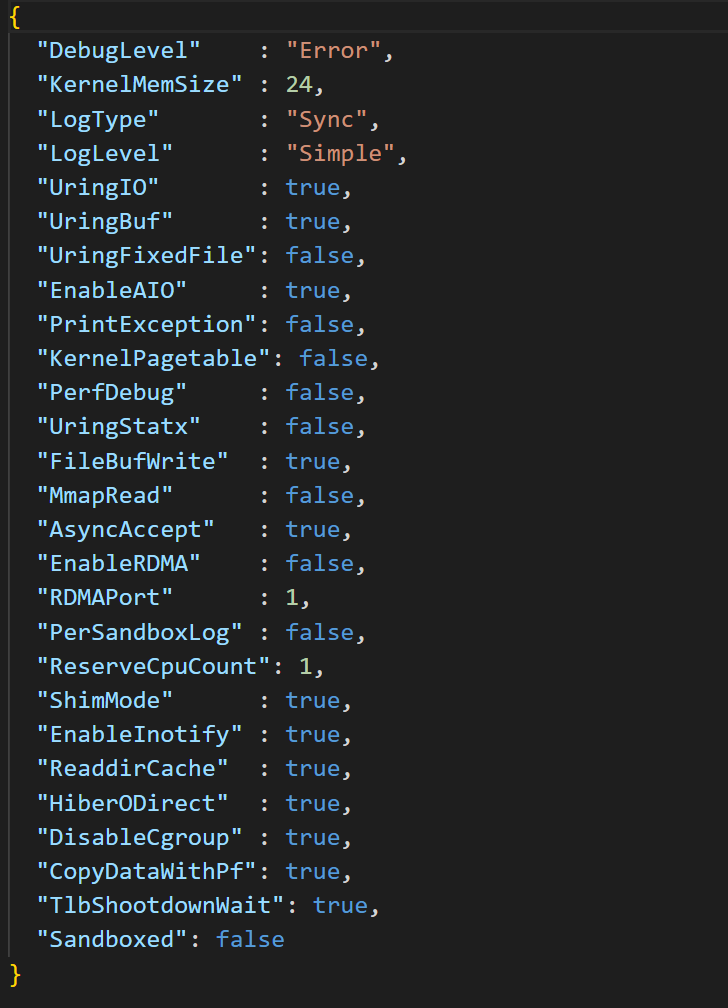
\includegraphics[width=0.3\textwidth]{images/quark_config.PNG}
%   \caption[Configuration file for Qkernel, Qvisor, and Quark Shim]{Configuration file for Qkernel, Qvisor, and Quark Shim. The file is installed as a global configuration file for Quark in the /etc/quark/ directory. When Quark Shim or Qvisor starts, it reads this file and completes the relevant configuration}
%   \label{fig:quark_config}
% \end{figure}

% Qkernel is a binary loaded into the guest memory during Qvisor setting up the guest. To properly configure the Qkernel, Qvisor also passes several command-line arguments to the Qkernel, including the number of VCPUs, the socket file descriptor that the Quark-agent listens to, and a configuration 
% file shown in Figure~\ref{fig:quark_config}. This configuration file specifies the runtime behavior of the Qkernel, such as whether to enable the Ucall interface, whether to enable RDMA, etc. A wrong configuration file can disclose the secrets stored in Qkernel. For example, turning on RDMA would allow an untrusted 
% party direct access to the Qkernel’s memory. For this reason, the Qkernel should measure the configuration file and send it to the relying party for integrity checking. For more details, please refer to section~\ref{sec:Enclave_Runtime_Measurement}.

% \subsection{Qkernel Log Misconfiguration}
% \label{sec:Qkernel_Log_Misconfiguration}
% Qkernel uses Hcall::HYPERCALL\_PRINT to store its logs under the host directory /var/log/quark. The Qkernel logging system supports five logging levels: OFF, Error, Info, Debug, and Trace. Here OFF is the minor level, i.e., the least detailed, and Trace is the highest level, i.e., the most detailed log. The user can configure the highest level of logging for 
% Qkernel through the DebugLevel keyword in the configuration file shown in Figure~\ref{fig:quark_config}. For example, when the DebugLevel is Info, Qkernel only prints logs in level Error and Info. 

% A malicious administrator may set the DebugLevel keyword to Trace and then analyze the Qkernel logs to obtain sensitive information. This problem can be solved by measuring the guest kernel arguments. However, both Qvisor and Qkernel are configured using this file. Specifically, Qvisor reads this configuration file after startup and passes a copy to the Qkernel when 
% launching the guest. In confidential computing, Qkernel and Qvisor belong to the application owner and the cloud provider, respectively. They have different interests and do not trust each other. For example, to resolve errors quickly, the cloud provider requires the log level in Qvisor to be set to TRACE, while the application owner 
% requires the log level in Qkernel to be OFF to protect the confidentiality of the \acrshort{CVM}. In the current architecture, Quark cannot satisfy both requirements. To this end, the Qkernel logging system configuration should be offloaded from the global configuration 
% file. The detail can be found in section~\ref{sec:Qkernel_logger}.




\section{Summary}
\label{sec:security_summarize}

This chapter first defines the threat model. Then, it analyzes the problems of the OCI runtime interface in confidential computing. A summary of the vulnerabilities found in the OCI runtime interface is listed in Section~\ref{sec:security_analyse_oci_summary}. Section~\ref{sec:security_analyse_quark_analysis} does a security analysis further on the Quark 
based on these vulnerabilities.
 
% \begin{enumerate}
%   \item \label{vulnerabilities:1} Application secrets are managed and deployed by untrusted Kubernetes and Quark Shim.
%   \item \label{vulnerabilities:2} Lack of cryptographic protection for interactive processes STDIN, STDOUT, and STDERR.
%   \item \label{vulnerabilities:3} Lack of cryptographic protection for non-interactive processes STDOUT and STDERR.
%   \item \label{vulnerabilities:4} Anyone can issue commands to an application.
%   \item \label{vulnerabilities:5} Any user can attach to an application.
%   \item \label{vulnerabilities:6} The commands issued by the application owner may contain confidential data but are unprotected during transmission.
%   \item \label{vulnerabilities:7} Loading compromised application binary during startup.
%   \item \label{vulnerabilities:8} Loading compromised binary/shared library at runtime.
%   \item \label{vulnerabilities:9}  Lack of management over application restart.
%   \item \label{vulnerabilities:10} No restriction to the available system calls for applications.
%   \item \label{vulnerabilities:11} No control over guest kernel arguments.
%   \item \label{vulnerabilities:12} Guest kernel log misconfiguration.

% \end{enumerate}

% For this reason, we should offload the configuration of the logging system from the qkernel configuration file and allow the application owner to specify the maximum logging level for the specified client kernel logging system in the protection 
% policy.
\cleardoublepage

